\documentclass[preprint,russian,a5paper,10pt,twoside,mediummath]{ncc}
\usepackage[utf8]{inputenc}
\usepackage{misccorr}			% различные особенности оформления документов, принятые в России
\usepackage{indentfirst}		% начинать абзац с красной строки
\usepackage{tikz}				% рисование чертежей
\usetikzlibrary{positioning}	% автоматическое размещение элементов на чертежах относительно друг друга
\usetikzlibrary{shapes.misc}
\usetikzlibrary{intersections}
\usepackage{enumitem}			% Для разрывов в списках
\usepackage{ncccomma}			% для использования запятой в качестве разделителя дробной части
\usepackage{framed}				% текст в рамке

\pagestyle{plain}
\countstyle{section}			% посекционная нумерация

%********Команда все примеры подчеркиваем
\newcommand{\ExampleMy}{\vspace{\baselineskip}\textbf{\underline{Пример:}}\nopagebreak\par}
%*********

\newcounter{problem}[section]				% счётчик примеров (имя example уже зарезервировано)
\renewcommand{\theproblem}{\thesection.\arabic{problem}}		% команда вывода текущего значения счётчика примеров
\newenvironment{problem}%	окружение для оформления примера
	{\par \vspace{\baselineskip} \refstepcounter{problem} {\raggedleft \textit{Пример \theproblem} \par} \vspace{-0.5\baselineskip} \begin{oframed}}%	это выполняется при отрытии окружения
	{\par \end{oframed}}%	а это при закрытии

\begin{document}

\begin{titlepage}
	\titlehead{\footnotesize САНКТ-ПЕТЕРБУРГСКИЙ\\ ГОСУДАРСТВЕННЫЙ ПОЛИТЕХНИЧЕСКИЙ УНИВЕРСИТЕТ\par\vspace{1mm} ИНСТИТУТ ИНФОРМАЦИОННЫХ ТЕХНОЛОГИЙ И УПРАВЛЕНИЯ\par\vspace{1mm} КАФЕДРА КОМПЬЮТЕРНЫХ СИСТЕМ\\ И ПРОГРАММНЫХ ТЕХНОЛОГИЙ}
	\titlefoot{Санкт-Петербург\\ \theyear}
	\author{С.\=,А.~Нестеров}
	\title{СИСТЕМЫ ОПТИМАЛЬНОГО УПРАВЛЕНИЯ}
	\titlecomment{Конспект лекций}
	\maketitle
\end{titlepage}

\bibindex{УДК \mbox{}\\ ББК \pbox[lt]{\mbox{} \\ \mbox{}}}
\copyrighttable{ISBN }
{	\item С.\=,А.~Нестеров, \theyear \\
	\item Санкт-Петербургский государственный\\ политехнический университет, \theyear }
\begin{abstract}
\fulltitle{Нестеров С.\=,А.}{\textbf{Системы оптимального управления}\=, : конспект лекций --- СПб.\=, : Изд-во политехнического ун-та, \theyear . --- \mbox{} с.}
Настоящее пособие представляет собой конспект лекций по первой части курса "<Оптимальное и адаптивное управление">, читаемого на кафедре "<Компьютерные системы и программные технологии"> для студентов пятого курса, обучающихся по профилю "<Встраиваемые системы управления">.

\begin{center}
\textbf{Редакторы:}\par Дмитрий Александрович Киселёв\\ Артур Константинович Еников
\end{center}

\end{abstract}

\newpage \setcounter{page}{3} \tableofcontents \newpage

\setcounter{secnumdepth}{-1}		% отключили нумерацию разделов
\section{Введение\label{intro}}
\setcounter{secnumdepth}{2}		% включили обратно

Для начала определимся, что понимается под управлением. Существует три фундаментальных принципа управления:
\begin{itemize}
\item Управление по заданию --- необходимо получить заданный сигнал $v$ на выходе объекта управления (ОУ). Для этого передаточная функция системы управления в целом (см. рис.~\ref{fig:intro:control_by_target}) должна быть равна единице. Тогда передаточная функция уст\-ройства управления (УУ) равна:
\begin{equation}\label{equ:intro:control_by_target}
W_{\text{\textit{УУ}}}=\frac{1}{W_{\text{\textit{ОУ}}}}
\end{equation}

\begin{figure}[ht] \centering		% [ht] - размещение в указанном месте, а если невозможно, то вверху следующей страницы
\begin{tikzpicture}											% здесь размеры по умолчанию в см
	[	auto,												% чтобы элементы чертежа не пересекались
		inner sep = 2ex,									% пространство, оставляемое вокруг текста
		block/.style={rectangle,draw=black,thick},		% стиль отрисовки блока
		vec/.style={->,>=stealth,semithick},				% стиль отрисовки вектора
		point/.style={inner sep = 0pt}	]
	\node[block] (object) {$ W_{\text{\textit{ОУ}}} $};	% Ставить ; обязательно! ИНАЧЕ ВСЁ ВИСНЕТ!!!!1
	\node[block] (regulator) [left = of object] {$ W_{\text{\textit{УУ}}} $};
%	\draw[vec] (regulator) to (object);					% вектор без подписи
	\draw[vec] (regulator) to node{$u$} (object);			% вектор с подписью
	\node[point] (input) [left = of regulator] {};
	\draw[vec] (input) to node{$v$} (regulator);
	\node[point] (output) [right = of object] {};
	\draw[vec] (object) to node{$x$} (output);
\end{tikzpicture}
\footnotesize \caption{Управление по заданию\label{fig:intro:control_by_target}}
\end{figure}

\item Управление по возмущению --- возмущения $f$, действующие на объект, учитываются при формировании управляющего воздействия $u$ (см. рис.~\ref{fig:intro:control_by_noise}). Передаточная функция от возмущений к выходу может быть выражена как $ W_{fu}W_\text{\textit{ОУ}}+W_{fx} $ и должна быть равна нулю. Тогда передаточная функция от возмущений к управлению равна:
\begin{equation}\label{equ:intro:control_by_noise}
W_{fu}=-\frac{W_{fx}}{W_\text{\textit{ОУ}}}
\end{equation}

\begin{figure}[ht] \centering
\begin{tikzpicture}	
	[	auto, inner sep = 2ex,
		block/.style={rectangle,draw=black,thick},
		vec/.style={->,>=stealth,semithick},
		point/.style={inner sep = 0pt}	]
	\node[block] (object) {$ W_\text{\textit{ОУ}} $};
	\node[block] (regulator) [left = of object] {$ W_\text{\textit{УУ}} $};
	\draw[vec] (regulator) to node{$u$} (object);
	\node[point] (input) [left = of regulator] {};
	\draw[vec] (input) to node{$v$} (regulator);
	\node[point] (output) [right = of object] {};
	\draw[vec] (object) to node{$x$} (output);
	\node[point] (noise) [above = of object] {};
	\draw[vec] (noise) to node(f){$f$} (object);
	\draw[vec] (f.west) -| (regulator.north);
	\fill (f.west) circle (1pt);
\end{tikzpicture}
\footnotesize \caption{Управление по возмущению\label{fig:intro:control_by_noise}}
\end{figure}

\item Управление по ошибке --- на вход регулятора подаётся отклонение $e$ выходного сигнала объекта $x$ от сигнала задания $v$ (см. рис.~\ref{fig:intro:control_by_eps}). Если $e$ устремить к нулю, то передаточная функция от $e$ к $x$ должна устремиться к бесконечности, чтобы получить на выходе заданную величину:
\begin{equation}\label{equ:intro:control_by_eps}
W_\text{\textit{УУ}}W_\text{\textit{ОУ}}\longrightarrow\frac{x_\text{\textit{уст}}}{0}=\infty
\end{equation}

Этого можно добиться, например, введением в регулятор очень больших коэффициентов усиления или интегрирующих звеньев.

\begin{figure}[ht] \centering
\begin{tikzpicture}	
	[	auto, inner sep = 2ex,
		block/.style={rectangle,draw,thick},
		vec/.style={->,>=stealth,semithick},
		point/.style={inner sep = 0pt}	]
	\node[block] (object) {$ W_\text{\textit{ОУ}} $};
	\node[block] (regulator) [left = of object] {$ W_\text{\textit{УУ}} $};
	\draw[vec] (regulator) to node{$u$} (object);
	\node[circle,draw,thick,inner sep=0pt,minimum size=2ex] (sum) [left = of regulator] {};
	\draw[semithick] (sum.north west) -- (sum.south east);
	\draw[semithick] (sum.south west) -- (sum.north east);
	\fill (sum.center) -- (sum.south west) arc (-135:-45:1ex) -- cycle;
	\draw[vec] (sum) to node{$e$} (regulator);
	\node[point] (input) [left = of sum] {};
	\draw[vec] (input) to node{$v$} (sum);
	\node[point] (output) [right = of object] {};
	\draw[vec] (object) to node(x){$x$} (output);
	\node[point] (p1) [below=of sum] {};
	\draw (x.south) |- (p1.center) [vec] to (sum);
	\fill (x.south) circle (1pt);
\end{tikzpicture}
\footnotesize \caption{Управление по ошибке\label{fig:intro:control_by_eps}}
\end{figure}
\end{itemize}
% Смотри формулу~\eqref{equ:intro:control_by_target}, с.~\pageref{equ:intro:control_by_target}.
% А теперь смотри рисунок~\ref{fig:intro:control_by_target}, с.~\pageref{fig:intro:control_by_target}.

По решаемой задаче системы автоматического управления (САУ) можно разделить на системы:
\begin{itemize}
\item стабилизации
\item программного управления
\item слежения
\item оптимального управления
\item адаптивного управления (поисковые и самонастраивающиеся)
\end{itemize}

Анализ и синтез САУ предполагает, что кроме цели рассматривается путь решения задачи. Для этого используются различные показатели качества:
\begin{itemize}
\item Прямые:
	\begin{itemize}
	\item Статические: статизм, добротность;
	\item Динамические: время переходного процесса, перерегулирование, колебательность;
	\end{itemize}
\pagebreak
\item Косвенные:
	\begin{itemize}
	\item Корневые;
	\item Частотные;
	\item Интегральные.
	\end{itemize}
\end{itemize}

Существует два основных подхода к синтезу САУ:
\begin{enumerate}
\item Обеспечить заданные показатели качества;
\item Обеспечить наилучшее (оптимальное) в каком-либо определённом смысле качество управления для заданного объекта при конкретных условиях работы и ограничениях.
\end{enumerate}

Эти два подхода имеют право на жизнь и естественно широко применяются. При этом надо понимать, что второй подход даёт максимально возможный (в отличие от первого, который даёт минимально пригодный) результат. Однако, за предельно достижимое качество необходимо будет чем-то "<заплатить">. Поэтому должно быть оценено, что даёт выигрыш в качестве и чем за это надо "<заплатить">. Соответственно, дальнейшее и посвящено рассмотрению теоретических моментов по расчёту и реализации соответствующих систем.

При решении такой задачи естественно требовать от управляемого процесса (ОУ) выполнения условий полной управляемости и наблюдаемости.

\clearpage		% выводит все накопившиеся плавающие элементы, а затем завершает страницу

\section{Постановка задачи оптимального управления\label{task}}

В общем случае постановки задач оптимального управления характеризуются значительным разнообразием, что связано с тремя основными причинами:
\begin{itemize}
\item Конкретными "<условиями"> функционирования, к которым следует отнести:
\begin{itemize}
\item начальное (исходное) и конечное (требуемое) состояния ОУ с временной привязкой $X_{0}\left ( t_{0} \right )$, $X_\text{\textit{к}}\left ( t_\text{\textit{к}} \right )$;
\item взаимосвязи, присущие реальным процессам, в форме:
\begin{itemize}
\item алгебраических (голономных) уравнений $G\left(x,u\right)=0$,
\item дифференциальных (неголономных) уравнений\\ $\varphi \left( x,u,t \right)=\dot{x}-Ax+Bu=0$,
\item интегральных (изопериметрических) уравнений\\ $I\left( x,u,t \right)=\int\limits_{t_0}^{t_\text{\textit{к}}}{\varphi \left( x,u,t \right)dt=C}$;
\end{itemize}
\end{itemize}
\item Ограничениями на управляющие сигналы и переменные состояния $\underline{U}\le U\le \overline{U}$; $\underline{X}\le X\le \overline{X}$; $\sum\limits_{i=1}^{n}{u_{i}^{2}}\le A$
\item Математическим видом критерия оптимальности.
\end{itemize}

Выбор критерия не является формальным актом, он не предписывается какой-либо теорией, а полностью определяется содержанием задачи управления. В общем виде критерий записывается функционалом:
\begin{equation}\label{equ:task:criterion_general}
J \left( U, X, \underset{t_\text{\textit{к}} - t_0}{\mathop{T}} \, \right) = \Phi \left( \underset{X_0, \, X_\text{\textit{к}}}{\mathop{ X \left( T \right) }} , T \right) + \int\limits_{t_0}^{t_\text{\textit{к}}} F\bigl( X(t), U(t), t \bigr) \, dt,
\end{equation}
где $ \Phi \bigl( X(T), T \bigr) $ --- терминальная составляющая, характеризующая качество управления только по начальному и конечному состояниям ОУ (поэтому отсутствует $U$); $ F \bigl( X(t), U(t), t \bigr) $ --- подынтегральная целевая функция, характеризующая качество внутри интервала управления. Управление должно обеспечивать экстремальное значение критерия оптимальности $ U = \underset{U}{\mathop{extr}} \, J \left( X, U, T \right) $. \smallskip 

Вид критерия $ J( X, U, T) $ задаёт класс задач оптимальности:
\begin{enumerate}
\item Критерий максимального быстродействия (минимального времени реакции):
\begin{enumerate}
\item[а)] $ \Phi \bigl( X(T), T \bigr) = T = t_\text{\textit{к}} - t_0 , \quad F\bigl( X(t), U(t), t \bigr) \equiv 0 $  
\item[б)] $ \Phi \bigl( X(T), T \bigr) \equiv 0 , \quad F\bigl( X(t), U(t), t \bigr) = 1 \to \int\limits_0^T 1\,dt = T $
\end{enumerate}

%\begin{subequations}\label{equ:task:minT}
%\renewcommand{\theequation}{\theparentequation\asbuk{equation}}
%\begin{equation}\label{equ:task:minT_first}
%y = x
%\end{equation}
%\begin{equation}\label{equ:task:minT_second}
%z = x^2(C+1)
%\end{equation}
%\end{subequations}

\item Критерий минимального расхода управления (топлива):
\[ \Phi \bigl( X(T), T \bigr) \equiv 0 , \quad F \bigl( X(t), U(t), t \bigr) = R \left| U \right| = \sum\limits_{i=1}^{n}{ r_i \left| u_i \right| } \]
\item Критерий предельной точности (минимальной ошибки):
\[ \Phi \bigl( X(T), T \bigr) \equiv 0, \quad F \bigl( X(t), U(t), t \bigr) = X^TQX, \] где $X$ --- отклонение (ошибка) от заданного значения, $Q$ --- матрица весовых коэффициентов (важность каждой составляющей в общей ошибке).
\item Критерий минимума энергетических затрат:
\[ \Phi \bigl( X(T), T \bigr) \equiv 0, \quad F \bigl( X(t), U(t), t \bigr) = U^TRU = \sum\limits_{i=1}^{n}{r_i u_i^2} \] на интервале $ t_\text{\textit{к}} - t_0 = T $
\item Критерий терминального управления (задача мягкой посадки или система управления конечным положением):
\[ \Phi \bigl( X(T), T \bigr) \ne 0, \quad F \bigl( X(t), U(t), t \bigr) \equiv 0 \]
\end{enumerate}
\pagebreak
Часто используются смешанные варианты критериев:
\begin{enumerate}[resume]
\item Квадратичный критерий качества управления (предельной точности при минимуме энергетических затрат):
\[ \Phi \bigl( X(T), T \bigr) \equiv 0, \quad F \bigl( X(t), U(t), t \bigr) = X^TQX + U^TRU \]
\item Критерий максимального быстродействия при минимальном расходе топлива (для управления автономными ОУ):
\[ \Phi \bigl( X(T), T \bigr) \equiv 0, \quad F \bigl( X(t), U(t), t \bigr) = 1 + R\left|U\right| = 1 + \sum\limits_{i=1}^{n}{ r_i \left| u_i \right| } \]
\item Критерий минимизации энергетических затрат при фиксированном интервале времени и заданном состоянии: 
\[ J = X^T \left( T \right) S X \left( T \right) + \int\limits_0^T \left( X^TQX + U^TRU \right) \, dt \] 
\end{enumerate}

Постановки задачи с критерием общего вида (двумя слагаемыми) принято называть задачей в форме Больца; терминальные постановки (только первое слагаемое) --- в форме Майера; постановки только с интегралом (без первого слагаемого) --- в форме Лагранжа.

%Вывод первого раздела
В итоге: задачи оптимального управления являются задачами минимизации на множестве функций и могут быть решены методами классического вариационного исчисления. Однако, наличие ограничений в форме равенств (уравнения УП и ОУ) и особенно в форме неравенств (ограничения допустимых управлений и состояний) требует применения методов неклассического вариационного исчисления, к которым относятся принцип максимума Л.\=,С.~Понтрягина, метод динамического программирования Р.~Беллмана, метод моментов Н.\=,Н.~Красовского, симплекс-метод линейного программирования, метод нелинейного программирования Табака-Куо, Куна-Таккера, символьные методы решения нелинейных алгебраических (например, трансцендентных) уравнений и~т.\,п. (градиентные и методы прямого поиска).


%Часть 3 Теория решения задач на экстремум
\clearpage
\section{Теория решения задач на экстремум\label{extremum}}
Формально достаточно общие задачи на отыскание $\max$  или $\min$ функции записываются в виде $\underset{x}{\mathop{extr}} \, F \left( x \right) $, $ x \in X $, т.\=,е.~найти в множестве $X$ точку $x$, при которой скалярная функция векторного аргумента $F \left( x \right) $ принимает экстремальное значение. При этом точки $ x = {\left( x_1, x_2, \dots x_n \right)}^T \in X$ называют допустимыми, само множество может быть ограничено или $ X \in \mathop{R}^n $, а задача поиска $ \max \, F\left( x \right) $ сведена к задаче поиска $ \min \, { - F \left( x \right) }$. Точку $ x^* \in \mathop{X}^* $ такую, что $ F \left( x^* \right) \underset{\le}{\ge} F \left( x \in X, \, x \ne x^* \right) $ называют решением задачи на $ \underset{\min}{\max} $ (экстремум), а $ F \left( x^* \right) $ --- значением экстремума.

Для сложных функций в заданной области может быть несколько таких точек (локальные экстремумы, также называемые слабыми, и абсолютные экстремумы, также называемые сильными).

Для отыскания решения задачи без ограничений необходимо:
\begin{itemize}
\item выписать условия экстремума:
\begin{equation}\label{equ:extremum:general}
grad \, F \left( x \right) = \frac{\partial F\left( x \right)}{\partial x} = 0
\end{equation}
(для скалярного аргумента: $\frac{df}{dx}=0$ );
\item найти решения этих уравнений --- полученные решения называют стационарными точками;
\item отыскать среди них решения задачи или доказать, что его нет. Достаточным условием решения задачи на $\max$ ($\min$) является отрицательная (положительная) определённость матрицы вторых производных $ \frac{ \partial ^ 2 F \left( x \right) }{ \partial x ^ 2} $ --- матрицы Гессе.
\end{itemize}

%**********
%Надо как-то выделить текст
%**********
%Пример
%\par\ExampleMy 
\begin{problem}
$ \min \, F \left( x \right) = \frac{1}{2} \left( x_1^2 + 4x_2^2 \right) $
\[ \left\{ \begin{darray}{l}
   \frac{\partial F}{\partial x_1} = x_1 \nr
   \frac{\partial F}{\partial x_2} = 4x_2
\end{darray} \right. \equiv 0 \enskip \Rightarrow \enskip \left\{ \begin{darray}{l}
   x_1 = 0 \\
   x_2 = 0
\end{darray} \right. \enskip \Rightarrow \enskip
\frac{ \partial ^ 2 F }{ \partial x ^ 2} = \left| \begin{matrix} 1 & 0 \\ 0 & 4 \end{matrix} \right| \]
Положительная определённость может быть подтверждена вычислением собственных чисел ($ \lambda _ 1 = 1, \lambda _ 2 = 4 $) или анализом всех диагональных миноров ($ \Delta _ 1 = 1, \Delta _2 = 4 $). Это доказывает, что стационарная точка $ \left( 0, 0 \right) $ абсолютный (глобальный) $\min$.
\end{problem}
\begin{problem}
$ \min \, F \left( x \right) = x_1^2 - 2 x_1 x_2 + 4 x_2^2 $
\[ \left\{ \begin{darray}{l}
   \frac{\partial F}{\partial x_1} = 2 x_1 - 2 x_2 = 0  \nr
   \frac{\partial F}{\partial x_2} = -2 x_1 + 8 x_2 = 0
\end{darray} \right. \enskip \Rightarrow \enskip x^* = {\left( 0, 0 \right)}^T \]
Матрица Гессе $ \frac{ \partial ^ 2 F }{ \partial x^2 } =
\left| \begin{array}{@{}rr@{}} 	% выравнивание обоих столбцов по правому краю
	 2 & -2 \\
	-2 &  8
\end{array} \right| $ положительно определённая --- это достаточное условие $ \min \, F \left( x^* \right) = 0 $
\end{problem}
\begin{problem}
$ f(x) = x^3 \left( x^2 - 1 \right) \to extr; \quad -1 \le x \le 2 $
\[ \frac{\partial f}{\partial x} = 5x^4 - 3x^2 = 0 \enskip \Rightarrow \enskip x_1 = 0, x_2 = \sqrt{3/5}, x_3 = - \sqrt{3/5} \]
\[ \frac{\partial ^ 2 F }{\partial x^2} = 20x^2 - 6x \]
\[ \left\{ \begin{darray}{l}
	\frac{\partial ^ 2 F }{\partial x^2} \Big| _{x=x_1} = 0 \nr
	\frac{\partial ^ 2 F }{\partial x^2} \Big| _{x=x_2} = 6\sqrt{3/5} > 0 \enskip \Rightarrow \min \nr
	\frac{\partial ^ 2 F }{\partial x^2} \Big| _{x=x_3} = -6\sqrt{3/5} < 0 \enskip \Rightarrow \max
\end{darray} \right. \]
\[ f \left( x_1 \right) = 0; \enskip f \left( x_2 \right) = - \frac{6}{25} \sqrt{\frac{3}{5}} \approx - 0,2; \enskip f \left( x_3 \right) = \frac{6}{25} \sqrt{\frac{3}{5}} \approx 0,2\]
\[ f(-1) = 0; \enskip f(2) = 24 \]
\end{problem}

\begin{figure}[ht] \centering
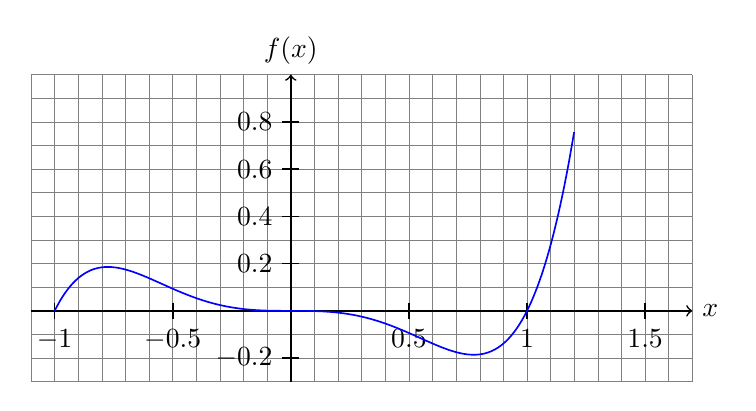
\begin{tikzpicture}
	[	scale=3,				% масштаб (относительно 1см)
		smooth,					% сглаживать углы
		samples=100,			% число точек на графике
		domain=-1:1.2	]		% диапазон значений входной величины
	\draw[very thin,gray,step=1 mm] (-1.1,-0.3) grid (1.7,1);		% сетка
	\draw[semithick,->] (-1.1,0) -- (1.7,0) node[right] {$x$};			% ось абсцисс
	\draw[semithick,->] (0,-0.3) -- (0,1) node[above] {$f(x)$};		% ось ординат
	\foreach \x in {-1,-0.5,0.5,1,1.5}
		\draw[semithick] (\x cm,1pt) -- (\x cm,-1pt) node[anchor=north] {$\x$};
	\foreach \y in {-0.2,0.2,0.4,0.6,0.8}
		\draw[semithick] (1pt,\y cm) -- (-1pt,\y cm) node[anchor=east] {$\y$};
	\draw[semithick,blue] plot (\x,{\x*\x*\x*(\x*\x-1)});		% график (ага, со степенями проблемы)
\end{tikzpicture}
\footnotesize \caption{График функции, рассмотренной в третьем примере\label{fig:extremum:third_example}}
\end{figure}

В качестве точек возможного экстремума необходимо проанализировать не только стационарные точки, но ещё границы допустимой области и точки возможных разрывов оптимизируемой функции.

При отыскания решения задачи с ограничениями в форме равенств $ X=\left\{ x \in \mathop{R}^n, G \left( x \right) = { \bigl( g_1(x), g_2(x),\ldots g_k(x) \bigr) }^T = 0 \right\} $ существует несколько методов. Наиболее просты и очевидны: метод прямой подстановки и метод составления функции Лагранжа. При решении методом составления функции Лагранжа необходимо:
\begin{itemize}
\item составить функцию Лагранжа:
\begin{equation}\label{equ:extremum:Lagrange}
L \left( x, \lambda \right) = F \left( x \right) + \lambda ^T G\left( x \right) ,
\end{equation}
где $ \lambda = { \left( \lambda _1, \lambda _2,\ldots \lambda _k \right) }^T $ --- вектор неопределённых множителей;
\item выписать необходимые условия экстремума $ \frac{\partial L}{\partial x} = 0, \enskip \frac{\partial L}{\partial \lambda } = 0 $;
\item найти стационарные точки и отыскать среди них решения задачи или доказать, что решения нет.
\end{itemize}

\begin{problem}
Найти стационарные точки для $F\left( x \right)=0.5\left( x_{1}^{2}+4x_{2}^{2} \right)$ при линейном ограничении на переменные $g\left( x \right)={{x}_{1}}+2{{x}_{2}}-1=0$.
\begin{itemize}
\item $L\left( x,\lambda  \right)=\frac{1}{2}\left( x_{1}^{2}+4x_{2}^{2} \right)+\lambda \left( {{x}_{1}}+2{{x}_{2}}-1 \right)$
\item Необходимые условия: $ \frac{\partial L}{\partial x_1} = x_1 + \lambda = 0 \enskip \Rightarrow \enskip x_1 = - \lambda ; \nr \frac{\partial L}{\partial x_2} = 4x_2 + 2\lambda = 0 \enskip \Rightarrow \enskip x_2 = - \frac{1}{2} \lambda ; \nr \frac{\partial L}{\partial \lambda } = x_1 + 2x_2 - 1 = 0 \enskip \Rightarrow \enskip \lambda = -0.5 $
\item Cтационарная точка: $ \bigl( x_1, x_2 \bigr) = \left( 0.5, 0.25 \right) $
\end{itemize}

\begin{align*}
\frac{\partial ^2 L}{\partial x_1^2} &= 1; & \frac{\partial ^2 L}{\partial x_1 \partial x_2} &= 0; & \frac{\partial ^2 L}{\partial x_1 \partial \lambda} &= 1 \nr
\frac{\partial ^2 L}{\partial x_2 \partial x_1} &= 0; & \frac{\partial ^2 L}{\partial x_2^2} &= 4; & \frac{\partial ^2 L}{\partial x_2 \partial \lambda} &= 2 \nr
\frac{\partial ^2 L}{\partial \lambda \partial x_1} &= 1; & \frac{\partial ^2 L}{\partial \lambda \partial x_2} &= 2; & \frac{\partial ^2 L}{\partial \lambda ^2} &= 0
\end{align*}

\[ \frac{{{\partial }^{2}}L}{\partial X, L} = \left| \begin{matrix}
   1 & 0 & 1  \\
   0 & 4 & 2  \\
   1 & 2 & 0 
\end{matrix} \right| = 1 \left| \begin{matrix}
   0 & 4  \\
   1 & 2 
\end{matrix} \right| - 2 \left| \begin{matrix}
   1 & 0  \\
   1 & 2 
\end{matrix} \right| = -8 \]
\[ F = \frac{1}{2} \left( { \left( \frac{1}{2} \right) }^2 + 4 { \left( \frac{1}{4} \right) }^2 \right) = \frac{1}{4} = F \left( x^* \right) \]
\[ F(x) = \frac{1}{2} \left( x_1^2 + 4x_2^2 \right) = C; \quad x_1^2 + 4x_2^2 = 2C = \frac{1}{2} \] 
\[ x_1 = \pm \frac{\sqrt{2}}{2} \approx 0.7; \quad x_2 = \pm \frac{\sqrt{2}}{4} \approx 0.35 \]
\end{problem}

% \ExampleMy
% \begin{enumerate}[resume]
% \item 

% \end{enumerate}

\begin{figure}[ht] \centering
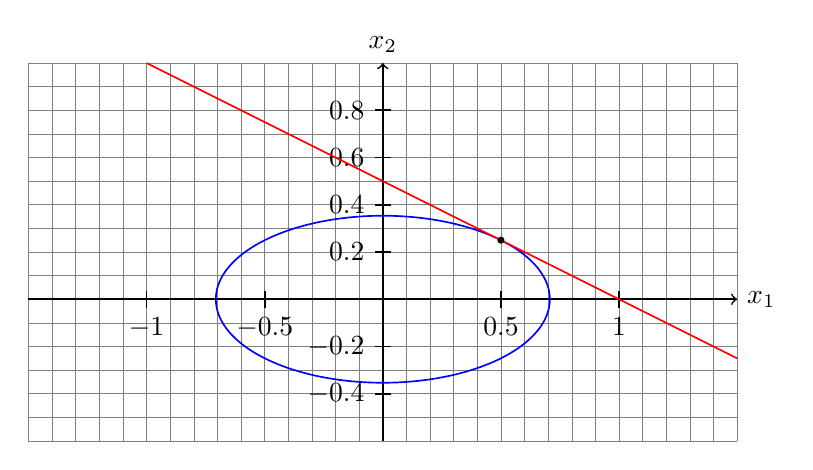
\begin{tikzpicture}[scale=3]
	\draw[very thin,gray,step=1 mm] (-1.5,-0.6) grid (1.5,1);
	\draw[semithick,->] (-1.5,0) -- (1.5,0) node[right] {$x_1$};
	\draw[semithick,->] (0,-0.6) -- (0,1) node[above] {$x_2$};
	\foreach \x in {-1,-0.5,0.5,1}
		\draw[semithick] (\x cm,1pt) -- (\x cm,-1pt) node[anchor=north] {$\x$};
	\foreach \y in {-0.4,-0.2,0.2,0.4,0.6,0.8}
		\draw[semithick] (1pt,\y cm) -- (-1pt,\y cm) node[anchor=east] {$\y$};
	\draw[semithick,blue,smooth cycle,variable=\t,samples=100,domain=-3.1415:3.1415]
		plot({cos(\t r)/sqrt(2)},{sin(\t r)/sqrt(8)});		% r значит радианы
	\draw[semithick,red] (-1,1) -- (1.5,-0.25);				% ограничение
	\fill (0.5,0.25) circle (0.15mm);							% стац. точка
\end{tikzpicture}
\footnotesize \caption{Решение задачи, рассмотренной в четвёртом примере\label{fig:extremum:fourth_example}}
\end{figure}

Задачи оптимизации без ограничений и с ограничениями в форме равенств называются классическими и могут быть решены аналитически. Все остальные (неклассические) очень редко могут решаться аналитически. Для их решения используют алгоритмы Куна-Таккера, градиентные методы, симплексные алгоритмы и методы прямого поиска.

Стационарные точки экстремальной задачи находятся путём решения уравнений вида $ Q(x) = 0 $, рекуррентным методом Ньютона. Последовательные приближения осуществляют по формуле $ x_{n+1} = x_n - \frac{ Q \bigl( x_n \bigr) }{ \Bigl(  dQ \bigl( x_n \bigr) / dx \Bigr) } $, геометрический смысл которой состоит в том, что точка $ x_{n+1} $ вычисляется как пересечение оси абсцисс с касательной к кривой $ y = Q(x) $ в точке $ x_n $.


\begin{problem}
Найти численное значение корня уравнения $ x - \sin x = \frac{ \pi }{2} $.\\
Составляем рекуррентную формулу:
\[ x_{n+1} = x_n - \frac{ x_n - \sin x_n - \pi/2}{ 1 - \cos x_n } \]
При ${{x}_{0}}=2.4$ получается итерационная последовательность:
\[ x_1 = 2.31, \enskip x_2 = 2.3099, \enskip x_3 = 2.309884, \ldots \]
\end{problem}


\clearpage
\section{Основы вариационного исчисления\label{variations}}
	\subsection{Оптимизация функционалов\label{variations:general}}

Функционал --- числовая скалярная функция, определяемая на множестве функций: $ y = f(x) $ --- функция от аргумента; $ J(x) = \int\limits_0^T F \left( x, \dot{x}, t \right) \, dt $ --- функция от функций  (скалярная оценка различных функций).

Каждая функция $ x(t) $ является точкой функционального пространства. Пусть эта функция однозначна, непрерывна и дифференцируема на рассматриваемом интервале (такие функции называются гладкими). Если значения функции соответствуют заданным в граничных точках их называют допустимыми. И тогда задача заключается в выборе среди допустимых функций такой, где функционал достигает наименьшего значения $ \underset{ x \in \Omega }{ \min } \, J(x) $. Решением таких задач занимается вариационное исчисление --- аналог дифференциального исчисления для функций.

Итак, для функций условиями экстремума являются:
\begin{gather*}
d \varphi (x) = 0 \quad \to \quad \delta J(x) = 0 \tag{*} \\
d^2 \varphi (x) \underset{\le}{\ge} 0 \quad \to \quad \delta ^2 J(x) \underset{\le}{\ge} 0 \tag{**}
\end{gather*}

Из условия $(*)$ выводится уравнение Эйлера:
\begin{equation}\label{equ:variations:Euler}
\frac{\partial F}{\partial x} - \frac{d}{dt} \left( \frac{\partial F}{\partial \dot{x}} \right) = 0
\end{equation}

Все функции удовлетворяющие этому уравнению, называются экстремалями. Если они проходят через граничные точки, то они называются допустимыми экстремалями.

Из условия $(**)$ выводятся условия Лежандра:
\begin{equation}\label{equ:variations:Legendre}
\frac{\partial ^2 F}{\partial \dot{x} ^2} \underset{\le}{\ge} 0
\end{equation}

\pagebreak

\begin{problem}
$J=\int\limits_0^1 \dot{x}^2 dt \to extr, \quad x(0) = 0, \enskip x(1) = 1 $
\[ F = \dot{x}^2 \enskip \Rightarrow \enskip \frac{\partial F}{\partial x} = 0, \enskip \frac{\partial F}{\partial \dot{x}} = 2\dot{x} \]
Уравнение Эйлера: $ \frac{\partial F}{\partial x} - \frac{d}{dt}\left( \frac{\partial F}{\partial \dot{x}} \right) = 0 \enskip \to \enskip 0 - \frac{d}{dt}\left( 2\dot{x} \right) = 0 $
\[ \ddot{x} = 0, \quad \dot{x} = C_1, \quad x = C_1 t + C_2 \]
\[ \left\{ \begin{darray}{l} x(0) = C_2 = 0 \\ x(1) = C_1 + C_2 = 1 \enskip \Rightarrow \enskip C_1 = 1 \end{darray} \right. \]
Допустимая экстремаль: $\hat{x}=t$\\
Условие Лежандра: $\frac{\partial ^2 F}{\partial \dot{x} ^2} = 2 > 0 \enskip \Rightarrow \enskip \min $
\[ J_{ \min } = \int\limits_0^1 { \left( \dot{\hat{x}} \right) }^2 dt = \int\limits_0^1 { \left( \dot{t} \right) }^2 dt = \int\limits_0^1 1^2 dt = t \Big|_0^1 = 1 \]
\end{problem}
\begin{problem}
Найти уравнение выхода $x(t)$  и характеристический полином СУ, для которой $ J(x) = \int\limits_{0}^{\infty } \left( a_0 x^2 + a_1 \dot{x} ^2 \right) \, dt \enskip \to \enskip \min $, при условиях $ a_0 > 0, a_1 > 0, x(0) = x_0, x( \infty ) = 0 $.
\[ F = a_0 x^2 + a_1 \dot{x} ^2, \quad \frac{\partial F}{\partial x} = 2 a_0 x, \quad \frac{\partial F}{\partial \dot{x}} = 2 a_1 \dot{x} \]
Уравнение Эйлера: $ 2 a_0 x - \frac{d}{dt} \left( 2 a_1 \dot{x} \right) = 0 $
\[ \ddot{x} - \frac{a_0}{a_1}x = 0, \quad \lambda ^2 - \frac{a_0}{a_1} = 0, \quad \lambda _{1, 2} = \pm \sqrt{\frac{a_0}{a_1}} \] 
\[ x(t) = C_1 e^{\sqrt{a_0 / a_1}\,t} + C_2 e^{-\sqrt{a_0 / a_1}\,t} \]
\[ \left. \begin{darray}{l} x(0) = C_1 + C_2 = x_0 \\
		x( \infty ) = C_1 \cdot \infty = 0 \enskip \Rightarrow \enskip C_1 = 0 \end{darray} \right\}
	\enskip \Rightarrow \enskip C_2 = x_0 \]
Допустимая экстремаль: $ \hat{x} = x_0 e^{-\sqrt{a_0 / a_1}\,t} $\\
Условие Лежандра: $\frac{\partial ^2 F}{\partial \dot{x} ^2} = 2 a_1 > 0 \enskip \Rightarrow \enskip \min $\\
Характеристический полином системы: $ D(p) = p + \sqrt{\frac{a_0}{a_1}} $ 
\end{problem}

Обобщим результаты в двух направлениях:
\begin{enumerate}
\item Многомерный случай: $ X = { \bigl( x_1(t), x_2(t), \ldots x_n(t) \bigr) }^T $ --- векторная функция.
\begin{equation}
\begin{gathered} J(X) = \int\limits_{t_0}^{t_\textit{к}} F \left( X, \dot{X}, t \right) \, dt \enskip \to \enskip \min \\
x_i(t_0) = x_{i0}, \enskip x_i(t_\textit{к}) = x_{i\textit{к}} \end{gathered}
\end{equation}
Тогда первое необходимое условие (уравнение Эйлера):
\begin{equation}
\frac{\partial F}{\partial {{x}_{i}}}-\frac{d}{dt}\left( \frac{\partial F}{\partial {{{\dot{x}}}_{i}}} \right) = 0, \quad i=\overline{1,n}
\end{equation}
Второе условие требует анализа матрицы вторых частных производных:
\[ \left\| \begin{array}{@{\,}cccc@{\,}}
	\frac{\partial ^2 F}{\partial \dot{x}_1^2} & \frac{\partial ^2 F}{\partial \dot{x}_1 \partial \dot{x}_2} & \ldots & \frac{\partial ^2 F}{\partial \dot{x}_1 \partial \dot{x}_n} \\[2ex]
	\frac{\partial ^2 F}{\partial \dot{x}_2 \partial \dot{x}_1} & \frac{\partial ^2 F}{\partial \dot{x}_2^2} & \ldots & \frac{\partial ^2 F}{\partial \dot{x}_2 \partial \dot{x}_n} \\[2ex]
	\hdotsfor[2.5]{4} \\[2ex]
	\frac{\partial ^2 F}{\partial \dot{x}_n \partial \dot{x}_1} & \frac{\partial ^2 F}{\partial \dot{x}_n \partial \dot{x}_2} & \ldots & \frac{\partial ^2 F}{\partial \dot{x}_n^2}
\end{array} \right\| \]
Для минимума все диагональные миноры должны быть $ \ge 0 $, для максимума $ \le 0 $. Строгие неравенства дают и достаточность условий.

%Непонятно что это пункт или часть случая
\begin{problem}
\[ J = \int\limits_0^1 \bigl( x_1 x_2 + \dot{x}_1 \dot{x}_2 \bigr) \,dt \enskip \to \enskip extr \]
\[ x_1(0) = x_2(0) = 1, \enskip x_1(1) = e, \enskip  x_2(1) = \frac{1}{e} \] 
\[ X = \bigl( x_1, x_2 \bigr) , \quad F = x_1 x_2 + \dot{x}_1 \dot{x}_2 \]
\[ \frac{\partial F}{\partial x_1} = x_2, \quad \frac{\partial F}{\partial \dot{x}_1} = \dot{x}_2 \enskip \Rightarrow \enskip \frac{\partial F}{\partial x_1} - \frac{d}{dt} \left( \frac{\partial F}{\partial \dot{x}_1} \right) = 0 \, : \enskip \ddot{x}_2 - x_2 = 0 \] \[ x_2 = C_1 e^t + C_2 e^{-t} \]
\[ \frac{\partial F}{\partial x_2} = x_1, \quad \frac{\partial F}{\partial \dot{x}_2} = \dot{x}_1 \enskip \Rightarrow \enskip \frac{\partial F}{\partial x_2} - \frac{d}{dt} \left( \frac{\partial F}{\partial \dot{x}_2} \right) = 0 \, : \enskip \ddot{x}_1 - x_1 = 0 \] \[ x_1 = C_3 e^t + C_4 e^{-t} \]
Подставив начальные и конечные условия, получим:
\[ \hat{x}_1 = e^t, \quad \hat{x}_2 = e^{-t} \]
\[ \left\| \begin{array}{@{\,}cc@{\,}}
	\frac{\partial ^2 F}{\partial \dot{x}_1^2} & \frac{\partial ^2 F}{\partial \dot{x}_1 \partial \dot{x}_2} \\[2ex]
	\frac{\partial ^2 F}{\partial \dot{x}_2 \partial \dot{x}_1} & \frac{\partial ^2 F}{\partial \dot{x}_2^2}
\end{array} \right\| = \left\| \begin{array}{@{\,}cc@{\,}}
	0 & 1 \\
	1 & 0
\end{array} \right\| \]
\[ \Delta _1 = 0, \enskip \Delta _2 = -1 \enskip \Rightarrow \enskip \max \]
\[ J_{\max } = \int\limits_0^1 \Bigl( e^t e^{-t} + e^t \bigl( {-e^{-t}} \bigr) \Bigr) \, dt = 0 \]
\end{problem}

\pagebreak
\item Задача со старшими производными:
\begin{equation}
\begin{gathered} J(x) = \int\limits_{t_0}^{t_\textit{к}} F \left( x, \dot{x}, \ddot{x}, \ldots x^{(n-1)}, t \right) \, dt \\
	x \bigl( t_0 \bigr) = x_0, \enskip \dot{x} \bigl( t_0 \bigr) = \dot{x}_0, \ldots \enskip x^{(n-1)} \bigl( t_0 \bigr) = x^{(n-1)}_0 \\
	x \bigl( t_\textit{к} \bigr) = x_\textit{к}, \enskip \dot{x} \bigl( t_\textit{к} \bigr) = \dot{x}_\textit{к}, \ldots \enskip x^{(n-1)} \bigl( t_\textit{к} \bigr) = x^{(n-1)}_\textit{к} \end{gathered}
\end{equation}

Существует два способа решения:
\begin{enumerate}
\item[а)] Рассматривается векторная функция, составляемая из исходной $ x(t) $ и её $ (n-1) $ производной, т.\=,е.~задача как многомерный случай.
\item[б)] Уравнение Эйлера преобразуется в уравнение Эйлера\-/Пу\-ассона:
\begin{equation}
\frac{\partial F}{\partial x} - \frac{d}{dt} \left( \frac{\partial F}{\partial \dot{x}} \right) + \frac{d^2}{dt^2} \left( \frac{\partial F}{\partial \ddot{x}} \right) - \ldots + {(-1)}^n \, \frac{d^n}{dt^n} \left( \frac{\partial F}{\partial x^{(n)}} \right) = 0
\end{equation}
Условие Лежандра: $ \frac{\partial ^2 F}{ { \left( \partial x^{(n)} \right) }^2 } \underset{\le}{\ge} 0 $

\begin{problem}
\[ J\left( x \right)=\int\limits_{0}^{1}{{{{\ddot{x}}}^{2}}}dt\enskip\to\enskip extr \]
\[ x\left( 0 \right)=\dot{x}\left( 0 \right)=0, \enskip x\left( 1 \right)=0, \enskip \dot{x}\left( 1 \right)=1 \]
\[ \begin{darray}{@{}l@{\qquad}l@{\qquad}}
F = \ddot{x}^2 \, : & \frac{\partial F}{\partial x} - \frac{d}{dt} \left( \frac{\partial F}{\partial \dot{x}} \right) + \frac{d^2}{dt^2} \left( \frac{\partial F}{\partial \ddot{x}} \right) = 0 \\
{} & \, 0 - 0 + \frac{d^2}{t^2} \left( 2 \ddot{x} \right) = 0 \enskip \Rightarrow \enskip x^{(4)} = 0
\end{darray} \]
\[ x^{(3)} = C_1, \quad \ddot{x} = C_1 t + C_2, \quad \dot{x} = \frac{1}{2} C_1 t^2 + C_2 t + C_3 \]
\[ x=\frac{1}{6}{{C}_{1}}{{t}^{3}}+\frac{1}{2}{{C}_{2}}{{t}^{2}}+{{C}_{3}}t+{{C}_{4}} \] 
\[ x(0) = C_4 = 0, \quad \dot{x} (0) = C_3 = 0 \]
\[ \left\{ \begin{darray}{l} x(1) = \frac{1}{6} C_1 + \frac{1}{2} C_2 = 0 \\
		\dot{x} (1) = \frac{1}{2} C_1 + C_2 = 0 \end{darray} \right. \enskip \Rightarrow \enskip
	\left\{ \begin{darray}{l} C_1 = 6 \\
		C_2 = -2 \end{darray} \right. \]
\[ \hat{x}={{t}^{3}}-{{t}^{2}}, \quad \ddot{\hat{x}}=6t-2 \] 
\[ J_{\min } = \int\limits_{0}^{1}{{{\left( 6t-2 \right)}^{2}}}dt = 12{{t}^{3}} \Big|_{0}^{1} - 12{{t}^{2}} \Big|_{0}^{1} + 4t \Big|_{0}^{1} = 4 \]
\end{problem}

\end{enumerate}
\end{enumerate}


\vspace{\baselineskip}
	\subsection{Задачи с нефиксированными границами\label{variations:floating_ends}}

Как для начального момента времени (левого конца), так и для конечного момента времени (правого конца) могут быть следующие варианты (для удобства будем рассматривать правый конец):
\begin{itemize}
\item Задача со \textit{свободным} правым концом --- $ t_\textit{к} $ не задано, $ x\bigl( t_\textit{к} \bigr) $ не задано.
\item Задача с \textit{подвижным} правым концом --- $ t_\textit{к} = T $, $ x\bigl( t_\textit{к} \bigr) $ не задано.
\item Задача со \textit{скользящим} правым концом --- $ t_\textit{к} $ не задано, $ x\bigl( t_\textit{к} \bigr) $ не задано, но определена их взаимосвязь $ x_\textit{к} = \psi \bigl( t_\textit{к} \bigr) $.
\end{itemize}

В этих случаях (когда отсутствует соответствующее граничное условие) необходимым условием экстремума, кроме уравнения Эйлера~\eqref{equ:variations:Euler}, становятся условия трансверсальности:
\begin{equation}
\left\{ \begin{array}{@{\,}r@{,\quad\text{если }}l}
	\left( F - \frac{\partial F}{\partial \dot{x}} \dot{x} \right) \Big|_{t=t_\textit{к}} = 0 & \text{не задано } t_\textit{к} \text{ и } x\bigl( t_\textit{к} \bigr) \\[2ex]
	\frac{\partial F}{\partial \dot{x}} \Big|_{t=t_\textit{к}} = 0 & \text{не задано } x\bigl( t_\textit{к} \bigr) \\[2ex]
	\biggl( F - \frac{\partial F}{\partial \dot{x}} \left( \dot{x} - \dot{\psi } \right) \biggr) \bigg|_{t=t_\textit{к}} = 0 & \text{конец скользящий}
\end{array} \right.
\end{equation}

В векторном случае --- $ X = { \bigl( x_1(t), x_2(t), \ldots x_n(t) \bigr) }^T $ --- необходимым условием достижения экстремума является система уравнений:
\begin{equation}
\left\{ \begin{array}{l}
	\frac{\partial F}{\partial x_i} - \frac{d}{dt} \left( \frac{\partial F}{\partial \dot{x}_i} \right) = 0, \quad i = \overline{1,n} \\[2ex]
	\begin{array}{@{}l@{\qquad}l@{}}
		\left( F - \sum\limits_{i=1}^{n} \frac{\partial F}{\partial \dot{x}_i} \dot{x}_i \right) \Bigg|_{t=t_0} = 0; &
		\left( F - \sum\limits_{i=1}^{n} \frac{\partial F}{\partial \dot{x}_i} \dot{x}_i \right) \Bigg|_{t=t_\textit{к}} = 0 \\[4ex]
		\frac{\partial F}{\partial \dot{x}_i} \Big|_{t=t_0} = 0, \quad i = \overline{1,n}; &
		\frac{\partial F}{\partial \dot{x}_i} \Big|_{t=t_\textit{к}} = 0, \quad i = \overline{1,n}
	\end{array}
\end{array} \right.
\end{equation}
Максимальное количество условий трансверсальности $2n+2$.

%\ExampleMy 
\begin{problem}
\[ J = \int\limits_{0}^{1}{\left( {{{\dot{x}}}^{2}}+x \right)\,dt}\enskip\to\enskip extr, \quad x\left( 1 \right)=0 \]
\[ \frac{\partial F}{\partial x}=1, \quad \frac{\partial F}{\partial \dot{x}}=2\dot{x}, \quad \text{уравнение Эйлера:} \enskip 1-\frac{d}{dt}\left( 2\dot{x} \right)=0 \]
\[ \text{условие трансверсальности:} \enskip 2\dot{x}\left( 0 \right) = 0 \]
\[ 1-2\ddot{x}=0, \quad \ddot{x}=\frac{1}{2}, \quad \dot{x}\left( t \right)=\frac{t}{2}+{{C}_{1}}, \quad x\left( t \right) = \frac{t^2}{4} + C_1 t + C_2 \]
\[ \dot{x} (0) = C_1  = 0, \quad x\left( 1 \right) = \frac{1}{4} + C_2 = 0 \enskip \Rightarrow \enskip C_2 = -\frac{1}{4} \]
\[ \hat{x}\left( t \right)=\frac{1}{4}\left( t^2 - 1 \right), \quad \dot{\hat{x}} = \frac{1}{2} t \]
\[ \frac{\partial ^2 F}{\partial \dot{x}^2} = 2 > 0 \enskip \Rightarrow \enskip \min \, : \quad J_{\min } = \int\limits_{0}^{1} \left( \frac{1}{4}{{t}^{2}}+\frac{1}{4}\left( {{t}^{2}}-1 \right) \right)\,dt = -\frac{1}{12} \] 
\end{problem}

Подводя итог, отмечаем, что необходимые условия минимизации функционалов представляются дифференциальными уравнениями относительно неизвестной функции (при минимизации функций не\-обходимые условия представляются алгебраическими уравнениями). Причём можно показать, что это нелинейное дифференциальное ура\-в\-нение второго порядка:
\[ \frac{\partial F}{\partial x}-\frac{d}{dt}\left( \frac{\partial F}{\partial \dot{x}} \right)=0, \quad \frac{d}{dt}\left( \frac{\partial F}{\partial \dot{x}} \right)=\frac{\partial }{\partial t}\frac{\partial F}{\partial \dot{x}} + \frac{\partial }{\partial x} \frac{dx}{dt} \frac{\partial F}{\partial \dot{x}} + \frac{\partial }{\partial \dot{x}} \frac{d\dot{x}}{dt} \frac{\partial F}{\partial \dot{x}} \]
\[ F = F\left( x, \dot{x}, t \right) ,\quad \frac{\partial F}{\partial \dot{x}}=\frac{\partial F}{\partial \dot{x}}\left( t,x,\dot{x} \right) \]
\[ \frac{\partial F}{\partial x} - \frac{\partial }{\partial t} \frac{\partial F}{\partial \dot{x}} - \frac{\partial ^2 F}{\partial \dot{x} ^2}\dot{x} - \frac{{{\partial }^{2}}F}{\partial {{{\dot{x}}}^{2}}}\ddot{x} = 0 \]

Уравнение Эйлера может приобретать частный вид:
\begin{enumerate}
\item[а)] если $ F\left( x,t \right) $ не зависит от $\dot{x}$, то $\frac{\partial F}{\partial x}=0$
\item[б)] если $F\left( \dot{x},t \right)$ не зависит от $x$, то $\frac{\partial F}{\partial \dot{x}}=const$ 
\item[в)] если $F\left( x,\dot{x} \right)$ не зависит от $t$, то $ F - \dot{x} \frac{\partial F}{\partial \dot{x}} = const $
\end{enumerate}

\vspace{\baselineskip}
	\subsection{Оптимизация функционалов с~ограничениями в~форме равенств\label{variations:conditional_extremum}}

При решении различных технических проблем нахождение экстремума требует учёта связей в форме алгебраических $ G(x,u)=0 $, дифференциальных $ \Phi (x,u,t) = \dot{x} - Ax - Bu = 0 $ и интегральных $ \int\varphi (x,u,t)dt = C $ уравнений, т.\=,е.~дополнительных условий. Тогда вместо функции $F\left( x, \dot{x}, t \right)$ берётся функция $L\left( x,u,t,\lambda  \right)=F\left( x,\dot{x},t \right) + \lambda ^T (t) \cdot \Phi \left( x,u,t \right)$ --- лагранжиан, где $ \lambda (t) $ --- вектор множителей Лагранжа, и уравнения приобретают вид Эйлера-Лагранжа:
\begin{equation}
\left\{ \begin{array}{l}
	\frac{\partial L}{\partial x} - \frac{d}{dt} \left( \frac{\partial L}{\partial \dot{x}} \right) = 0 \\[2ex]
	\frac{\partial L}{\partial u} - \frac{d}{dt} \left( \frac{\partial L}{\partial \dot{u}} \right) = 0
\end{array} \right.
\end{equation}

\pagebreak
\begin{problem}
Пусть динамическая система задана уравнениями:
\[ \left\{ \begin{array}{l}
	\dot{x}_1 = x_2 \\
	\dot{x}_2 = {-x_1} + u
\end{array} \right. \]
с произвольным начальным состоянием $ x_1(0), x_2(0) $ и нулевым конечным $ x_1( \infty ) = x_2( \infty ) = 0 $.
Требуется: \[ \min\int\limits_{0}^{ \infty } \bigl( x_1^2 + x_2^2 + 0.1u^2 \bigr) \, dt \]

\begin{enumerate}
\item Составляем лагранжиан:
\[ L( x, u, \lambda ) = \bigl( x_1^2 + x_2^2 + 0.1u^2 \bigr) + \lambda _1 \bigl( \dot{x}_1 - x_2 \bigr) + \lambda _2 \bigl( \dot{x}_2 + x_1 - u \bigr) \]
\item Составляем уравнения Эйлера-Лагранжа:
\[ \left\{ \begin{array}{l}
	\frac{\partial L}{\partial x_1} - \frac{d}{dt} \left( \frac{\partial L}{\partial \dot{x}_1} \right) = 2x_1 + \lambda _2 - \frac{d}{dt} \bigl( \lambda _1 \bigr) = 0 \\[2ex]
	\frac{\partial L}{\partial x_2} - \frac{d}{dt} \left( \frac{\partial L}{\partial \dot{x}_2} \right) = 2x_2 - \lambda _1 - \frac{d}{dt} \bigl( \lambda _2 \bigr) = 0 \\[2ex]
	\frac{\partial L}{\partial u} - \frac{d}{dt} \left( \frac{\partial L}{\partial \dot{u}} \right) = 0.2u - \lambda _2
\end{array} \right. \]
\end{enumerate}
Учитывая уравнения системы и исключая $ u $, получим:
\[ \dot{x}_1 = x_2, \quad \dot{x}_2 = - x_1 + 5 \lambda _2, \quad \dot{ \lambda }_1 = 2x_1 + \lambda _2, \quad \dot{ \lambda }_2 = - \lambda _1 + 2x_2 \]

\[ \left| \begin{matrix}
	\dot{x}_1 \\
	\dot{x}_2 \\
	\dot{ \lambda }_1 \\
	\dot{ \lambda }_2
\end{matrix} \right| = \underbrace{ \left| \begin{array}{rrrr}
	 0	& \hphantom{-}1		& 0		& \hphantom{-}0		\\
	-1	& 0					& 0		& 5					\\
	 2	& 0					& 0		& 1					\\
	 0	& 2					& -1	& 0
\end{array} \right| }_{A} \cdot
\left| \begin{matrix}
	x_1 \\
	x_2 \\
	\lambda _1 \\
	\lambda _2
\end{matrix} \right| \]

\[ \left| Ep-A \right| = \left| \begin{array}{rrrr}
   p & -1 & 0 & 0  \\
   1 & p & 0 & -5  \\
   -2 & 0 & p & -1  \\
   0 & -2 & -1 & p  
\end{array} \right| = p^4 - 8p^2 + 11 \]
\[ p_{1,2} = \pm 2.5, \quad p_{3,4} = \pm 1.32 \]

Зная, что условию устойчивого решения отвечают только левые корни, ищем решение в виде:
\[ x_1(t) = C_1 e^{-2.5t} + C_2 e^{-1.32t} + \underbrace{ C_3 e^{2.5t} + C_4 e^{1.32t} }_{ x\left( \infty  \right) = 0 } \]
\[ x_2 = \dot{x}_1 = -2.5 \, C_1 e^{-2.5t} - 1.32 \, C_2 e^{-1.32t} \]
\[ \dot{x}_2 = 6.25 \, C_1 e^{-2.5t} + 1.75 \, C_2 e^{-1.32t} \]
\[ u = \dot{x}_2 + x_1 = 3.75 \, C_1 e^{-2.5t} + 0.43 \, C_2 e^{-1.32t} \]

\[ \left| \begin{matrix}
	x_1 \nr
	x_2
\end{matrix} \right| = \left| \begin{array}{cc}
	1 & 1  \nr
	-2.5 & -1.32
\end{array} \right| \cdot \left| \begin{matrix}
	C_1 e^{-2.5t} \nr
	C_2 e^{-1.32t}
\end{matrix} \right| \]

\[ \left| \begin{array}{@{}c@{}}
	C_1 e^{-2.5t} \nr
	C_2 e^{-1.32t}
\end{array} \right| = \left| \begin{array}{rr}
   -1.12 & -0.85  \nr
   2.12 & 0.85
\end{array} \right| \cdot \left| \begin{array}{@{}c@{}}
	x_1 \nr
	x_2
\end{array} \right| \]

\[ u = \left( \begin{array}{@{\,}c@{;\enskip}c@{\,}} 3.75 & 0.43 \end{array} \right) \cdot \left( \begin{array}{@{\,}rr@{\,}}
   -1.12 & -0.85  \nr
   2.12 & 0.85
\end{array} \right) \cdot \left( \begin{matrix}
	x_1 \nr
	x_2
\end{matrix} \right) = -3.2x_1 - 2.8x_2 \]

\end{problem}

\vspace{\baselineskip}
	\subsection{Каноническая (Гамильтонова) форма уравнений Эйлера (Лагранжа)\label{variations:Canonical_Euler}}
	
Стремление избавится от двойного дифференцирования (по времени $ \frac{d}{dt} $ и по производным $ \frac{\partial }{\partial \dot{x}} $ состояния и $ \frac{\partial }{\partial \dot{u}} $ управления) привело к предложению ввести канонические переменные $ \psi _i (t) $, сопряжённые с переменными состояния ОУ, и функцию Гамильтона:
\begin{gather}
H = - F(x,u,t) + \sum\limits_{i=1}^{n} \psi _i \dot{x}_i, \quad \psi _i = \frac{\partial F}{\partial \dot{x}_i} \\
H = - L(x,u, \lambda ,t) + \sum\limits_{i=1}^{n} \psi _i \dot{x}_i, \quad \psi _i = \frac{\partial L}{\partial \dot{x}_i}
\end{gather}
Учитывая, что:
\[ \frac{\partial H}{\partial x_i} = - \frac{\partial F}{\partial x_i} = - \frac{\partial H}{\partial x_i}, \quad \dot{x}_i = \frac{dx_i}{dt} = \frac{\partial H}{\partial \psi _i} \]
\[ \frac{\partial F}{\partial x_i} - \frac{d}{dt} \Bigl( \underbrace{ \frac{\partial F}{\partial \dot{x}_i} }_{\psi _i} \Bigr) = 0 \enskip \Rightarrow \enskip \frac{d}{dt} \psi _i = \frac{\partial F}{\partial x_i} \]
Получаем систему уравнений:
\begin{equation}
\left\{ \begin{darray}{l}
   \frac{dx_i}{dt} = \frac{\partial H}{\partial \psi _i}, \quad i=\overline{1,n} \nr
   \frac{d\psi _i}{dt} = - \frac{\partial H}{\partial x_i}, \quad i=\overline{1,n} \nr
   \frac{\partial H}{\partial u_j} = 0, \quad j=\overline{1,m}
\end{darray} \right.
\end{equation}
При условии, что в уравнении ОУ $\dot{x}=Ax+Bu$ отсутствуют производные управления $\dot{u}$.

При нефиксированных граничных условиях уравнения трансверсальности в канонической форме имеют вид:
\begin{equation}
\left\{ \begin{darray}{l@{\quad}l}
   {{\psi }_{i}}\left( {{t}_{0}} \right)=0, & \psi _i \bigl( t_\textit{к} \bigr) = 0 \\
   H\left( {{t}_{0}} \right)=0, & H \bigl( t_\textit{к} \bigr) = 0
\end{darray} \right.
\end{equation}

Такая форма уравнений даёт большое преимущество, т.\=,к.~слева только дифференцирование по времени, а справа частные производные по переменным.

Для общей задачи Лагранжа канонические переменные $ \psi (t) $ совпадают с неизвестными множителями Лагранжа $ \lambda (t) $.

Кроме того, переход к функции Гамильтона позволяет снизить требования к гладкости изменения переменных состояния и управления и решать задачи в условиях ограничений в виде неравенства.

Для консервативных механических систем функция Гамильтона $H$ имеет простой физический смысл --- она совпадает с полной механической энергией, и равенство $H=const$ имеет смысл закона сохранения полной механической энергии.

В общем случае для линейного объекта в форме уравнений состояния $\dot{x}=Ax+Bu$ ($n$-размерности), в котором отсутствует зависимость от $\dot{u}$, уравнения вариационной задачи записываются в следующем виде:
\begin{equation}
\left\{ \begin{darray}{l}
	\frac{\partial X}{\partial t} = \left\| \frac{\partial H}{\partial \lambda _i} \right\| = AX + BU = \Phi _1, \quad i=\overline{1,n} \\
	\frac{\partial \lambda }{\partial t} = - \left\| \frac{\partial H}{\partial x_i} \right\| = \left\| \frac{\partial F}{\partial x_i} \right\| + \lambda ^T \left\| \frac{\partial \Phi _1}{\partial x_i} \right\|, \quad i=\overline{1,n} \\
	\frac{\partial H}{\partial u_j} = \frac{\partial F}{\partial u_j} + \sum\limits_{i=1}^{n} \lambda _i \frac{\partial \varphi _{1i}}{\partial u_j} = 0, \quad j=\overline{1,r}
\end{darray} \right.
\end{equation}

\begin{problem}
Определим оптимальное управление объектом:
\[ T\dot{x}+x=ku, \quad \frac{x}{u}=\frac{k}{Tp+1} \enskip \Rightarrow \enskip \dot{x}=-\frac{1}{T}x+\frac{k}{T}u=ax+bu \]
\[ J=\int\limits_{0}^{\infty }{\left( q{{x}^{2}}+r{{u}^{2}} \right)} \, dt \enskip \Rightarrow \enskip L = qx^2 + ru^2 + \lambda \left( \dot{x} - ax - bu \right) \]
\[ H = -q{{x}^{2}}-r{{u}^{2}}+\lambda \left( ax+bu \right) \]
\[ \left\{ \begin{darray}{l}
   \dot{x}=\frac{\partial H}{\partial \lambda }=ax+bu  \\
   \dot{\lambda }=-\frac{\partial H}{\partial x} = 2qx - \lambda a  \\
   0 = -\frac{\partial H}{\partial u}=2ru-\lambda b \enskip \Rightarrow \enskip u=\frac{b}{2r}\lambda
\end{darray} \right. \]

\[ \left\{ \begin{darray}{l}
   \dot{x}=ax+\frac{{{b}^{2}}}{2r}\lambda   \\
   \dot{\lambda }=2qx-a\lambda
\end{darray} \right. = \left| \begin{darray}{c@{\quad}c}
   a & \frac{{{b}^{2}}}{2r}  \\[1ex]
   2q & -a  
\end{darray} \right| \cdot \left| \begin{darray}{c}
   x  \\[1ex]
   \lambda  
\end{darray} \right| \]

\pagebreak
Для определения корней системы составим определитель:
\[ \Delta (p) = \left| Ep-A \right| = \left| \begin{darray}{c@{\quad}c}
   p-a & -\frac{{{b}^{2}}}{2r}  \\[1ex]
   -2q & p+a  
\end{darray} \right| = p^2 - \left( a^2 + q\frac{b^2}{r} \right) = 0 \]
\[ p_{1,2} = \pm \sqrt{ a^2 + q\frac{b^2}{r} } \]

Условию устойчивости удовлетворяет только отрицательный корень, поэтому решение ищем в виде:
\[ \left\{ \begin{darray}{l}
   x = C_1 e^{p_2t} \\
   \lambda = C_2 e^{p_2t}
\end{darray} \right. \]
\[ C_1 = x_0, \quad C_2 = \frac{ \left( p_2 - a \right) 2r }{b} C_1 = \frac{2q}{p_2 + a} C_1 \]

Следовательно, искомое оптимальное управление:
\[ u_\textit{опт} (t) = \frac{b}{2r} \lambda (t) = \frac{bq}{r\left( p_2 - a \right)} \cdot \underbrace{ C_1 e^{p_2t} }_{x(t)} = \frac{p_2-a}{b} \underbrace{ C_1 e^{p_2t} }_{x(t)} = \underbrace{ \frac{p_2-a}{b} }_{K_\textit{опт}} x(t) \]

Такое решение определяет структуру оптимального регулятора в форме отрицательной пропорциональной обратной связи:
\[ K_\textit{опт} = \frac{p_2-a}{b} = -\frac{a+\sqrt{a^2+qb^2/r}}{b} \]
   
\end{problem}

Вспоминая пример поиска характеристического полинома системы $D\left( p \right)=p+\sqrt{\frac{{{a}_{0}}}{{{a}_{1}}}}\,$, доставляющего $\min \, J=\int\limits_{0}^{\infty }{\left( a_0{{x}^{2}}+a_1{{{\dot{x}}}^{2}} \right)} \, dt$, перепишем его в нашем случае:
\begin{multline*}
J = \int\limits_{0}^{\infty }{\Bigl( q{{x}^{2}}+r{{u}^{2}} \Bigr)} \, dt = \int\limits_{0}^{\infty }{\left( q{{x}^{2}}+r{{\left( \frac{\dot{x}-ax}{b} \right)}^{2}} \right)} \, dt ={} \\*
	\int\limits_{0}^{\infty }{ \Biggl[ \left( q+r\frac{{{a}^{2}}}{{{b}^{2}}} \right){{x}^{2}}-\frac{2ra}{{{b}^{2}}}x\dot{x}+\frac{r}{{{b}^{2}}}{{{\dot{x}}}^{2}} \Biggr] } \, dt
\end{multline*}
\[ F=\left( q+r\frac{{{a}^{2}}}{{{b}^{2}}} \right){{x}^{2}}-\frac{2ra}{{{b}^{2}}}x\dot{x}+\frac{r}{{{b}^{2}}}{{\dot{x}}^{2}} \]
\[ \frac{\partial F}{\partial x}=2\left( q+r\frac{{{a}^{2}}}{{{b}^{2}}} \right)x-\frac{2ra}{{{b}^{2}}}\dot{x}, \quad
	\frac{\partial F}{\partial \dot{x}}=-\frac{2ra}{{{b}^{2}}}x+\frac{2r}{{{b}^{2}}}\dot{x} \]
Уравнение Эйлера:
\[ \frac{\partial F}{\partial x}-\frac{d}{dt}\left( \frac{\partial F}{\partial \dot{x}} \right)=0 \enskip \Rightarrow \enskip 2\left( q + r \frac{a^2}{b^2} \right) x - \frac{2ra}{b^2} \dot{x} + \frac{2ra}{b^2} \dot{x} - \frac{2r}{b^2} \ddot{x} = 0 \]
\[ \ddot{x} - \left( a^2 + q \frac{b^2}{r} \right) x = 0 \]
Соответствующий характеристический полином \vspace{1ex} ${{p}^{2}}-\left( {{a}^{2}}+q\frac{{{b}^{2}}}{r} \right)=0$ можно представить как $\left[ p^2 - \sqrt{a^2 + q \frac{b^2}{r}} \right] \cdot \left[ p^2 + \sqrt{a^2 + q \frac{b^2}{r}} \right] = 0 $ \vspace{1ex} --- произведение полиномов с симметричным расположением левого и правого полюсов --- это \textit{факторизация}. Устойчивый характер процессов даёт полином $ p^2 + \sqrt{a^2 + q \frac{b^2}{r}} = 0 $.

Если мы ищем оптимальную обратную пропорциональную связь для объекта $\dot{x}=ax+bu$, то $ u_\textit{опт} = K_\textit{опт} \cdot x $, $\dot{x}=ax+b{{K}_\textit{ос}}x=\left( a+b{{K}_\textit{ос}} \right)x$ и $D\left( p \right)=p-\left( a+b{{K}_\textit{ос}} \right)$. Приравнивая два полинома $p+\sqrt{{{a}^{2}}+q\frac{{{b}^{2}}}{r}}=p-\left( a+b{{K}_\textit{ос}} \right)$, получим:
\[ K_\textit{ос} = \frac{-\sqrt{{{a}^{2}}+q\frac{{{b}^{2}}}{r}}-a}{b} \]
Как видно, решения совпадают. В литературе принято такой подход называть синтезом линейного оптимального регулятора в частотной области.

Записывая факторизацию для $D(p)$, получим:
\[ \Bigl[ p - \bigl( a+b{{K}_\textit{ос}} \bigr) \Bigr] \cdot \Bigl[ p + \bigl( a+b{{K}_\textit{ос}} \bigr) \Bigr] = {{p}^{2}}-\left( {{a}^{2}}+q\frac{{{b}^{2}}}{r} \right) \]
\[ {{p}^{2}}-{{\left( a+b{{K}_\textit{ос}} \right)}^{2}}={{p}^{2}}-\left( {{a}^{2}}+\frac{{{b}^{2}}}{r}q \right) \]
\begin{equation}\label{equ:variations:Riccati}
K_\textit{ос}^2 + \frac{2a}{b} K_\textit{ос} - \frac{q}{r} = 0
\end{equation}
Это скалярное стационарное уравнение Риккати. В итоге получаем:
\[ K_\textit{ос} = -\frac{a}{b}\pm \sqrt{\frac{{{a}^{2}}}{{{b}^{2}}}+\frac{q}{r}} \]

\clearpage
\section{Принцип максимума\label{maximum}}
	\subsection{Определение\label{maximum:def}}
В целом ряде практических задач оптимизацию функционала при заданных дифференциальных (динамических) уравнениях объекта $\left\{ \dot{X}=\Phi \left( x,u \right)=AX+BU \right\}$ требуется обеспечивать при ограниченных диапазонах допустимого изменения управлений $\left| {{u}_{i}} \right|\le {{U}_{i}}$   и/или координат объекта $\left| {{x}_{i}} \right|\le {{X}_{i}}$. В изменениях функций образуются переломы, в изменении производных --- разрывы. Нарушаются условия, при которых были выведены уравнения Эйлера и Эйлера\-/Лагранжа в вариациях.

Коллективом ученых под руководством академика Л.\=,С.~Понтрягина (В.\=,Г.~Болтянский, Р.\=,В.~Гамкрелидзе, Е.\=,Ф.~Мищенко и др.) был разработан принцип максимума, использующий понятие игольчатой вариации относительно оптимального управления и траектории движения, что позволило доказать применимость модифицированной функции Гамильтона для таких неклассических вариационных задач. Модификация заключалась в следующем:
\begin{itemize}
\item уравнение для критерия качества $J=\int\limits_{{{t}_{0}}}^{{{t}_\textit{к}}}{{{F}_{0}}\left( x,u \right) \, dt}$ из интегральной формы преобразовывалось в дифференциальную
\begin{equation}
\dot{x}_0 = \dot{F}_0 (x,u), \quad x_0 = J \big|_{t_0}^{t_\textit{к}}
\end{equation}
\item формирование расширенного вектора ${{\left[ {{x}_{0}},x \right]}_{n+1}}$ и новой функции Гамильтона
\begin{equation}
{{H}^{*}}\left( {{\psi }_{0}},\psi ,x,u \right)={{\psi }_{0}}{{F}_{0}}\left( x,u \right)+{{\psi }^{T}}\Phi \left( x,u \right)=\sum\limits_{i=0}^{n}{{{\psi }_{i}}{{f}_{i}}\left( x,u \right)}\,,
\end{equation}
где ${{\psi }_{0}}=-1$ для перехода от минимизации $J$ к максимизации $H$.
\end{itemize}

\pagebreak
Канонические уравнения Гамильтона тогда имеют вид:
\begin{equation}
\left\{ \begin{darray}{l}
   \frac{d{{x}_{i}}}{dt}=\frac{\partial {{H}^{*}}}{\partial {{\psi }_{i}}}, \enskip i=\overline{0,n}  \\
   \frac{\partial {{\psi }_{i}}}{dt}=-\frac{\partial {{H}^{*}}}{\partial {{x}_{i}}}, \enskip i=\overline{0,n}  \\
   \frac{\partial H^*}{\partial u}=0
\end{darray} \right.
\end{equation}
Их количество $2n+2+r$, и решение задачи при фиксированных начальной $ x \bigl( t_0 \bigr) $ и конечной $ x \bigl( t_\textit{к} \bigr) $ точках даётся следующей теоремой.

\begin{theorem}[(Л.\=,С.~Понтрягин, 1956~г.)]
Для того, чтобы допустимое управление $ u^* (t) $ и соответствующая ему траектория $ x^* (t) $ были оптимальными необходимо существование такой ненулевой непрерывной векторной функции $ \psi ^* (t) $, отвечающей в силу уравнений Гамильтона функциям  $ u^* (t) $ и $ x^* (t) $, что:
\begin{enumerate}
\item в любой момент времени $ t_0 \le t \le t_\textit{к} $, когда $ u^* (t) $ непрерывна, функция $ H^* \left( x^*, u^* \right) = \underset{u \in U}{ \max } \, H^* \left( \psi _0^*, \psi ^*, x^*, u \right) $ достигает максимума;
\item в любой момент времени $ \psi _0^* = -1, \enskip H^* \bigl( \psi ^* (T), x^* (T) \bigr) = 0 $.
\end{enumerate}
\end{theorem}

При этом наличие разрывов в изменении производных накладывает дополнительные условия ($ t_0^* $ --- точка разрыва):
\[ \begin{darray}{l} \left. \!\!
	\begin{darray}{l}
		\psi _i \bigl( t_{+0}^* \bigr) = \psi _i \bigl( t_{-0}^* \bigr) \\
		H \bigl( t_{+0}^* \bigr) = H \bigl( t_{-0}^* \bigr)
	\end{darray} \right\} \enskip \text{условия Вейерштрасса-Эрдмана,} \\
	x_i \bigl( t_{+0}^* \bigr) = x_i \bigl( t_{-0}^* \bigr) \enskip \text{\mbox{} --- условия припасовывания.}
\end{darray} \]

Конструктивный вид этой теоремы позволяет построить алгоритмическую процедуру определения оптимального управления:
\begin{enumerate}
\item Составить гамильтониан системы:
\[ H(\psi , x, u) = -F(x,u) + \psi ^T \Phi (x,u) \]
\item Максимизировать его по $ u(t) \in U $:
\[ \underset{u \in U}{ \max } \, H^* ( \psi ^*, x^*, u ) = H^* ( \psi ^*, x^* ), \]
определяя управление как функцию вектора состояния и вспомогательной переменной: $ u^* = u ( \psi ^*, x^* ) $
\item Составить систему однородных дифференциальных уравнений для вспомогательной переменной:
\[ \dot{\psi } = -\frac{\partial H}{\partial x} \]
\item Решить эту систему уравнений при неизвестных начальных условиях и заданных соответствующим сопряжённой системе условиям для $ x \bigl( t_0 \bigr) $ и $ x \bigl( t_\textit{к} \bigr) $ --- краевым или условиям трансверсальности. Соответствующее решение ищется аналитически или численными методами.
\end{enumerate}

Для неконсервативных систем $ H^* = \psi \dot{X} $ будет мощностью, а $ \psi _i $ \--- импульсами воздействий, которые вводят в ОУ такое количество энергии, которое обеспечивало бы заданный закон движения и экстремум функционала критерия качества.

\begin{problem}
\[ \min \, J = \int\limits_0^4 \bigl( x + u^2 \bigr) \, dt, \quad \dot{x} = u, \quad x(4) = 0, \quad |u| \le 1 \]
\begin{enumerate}
\item $ H\left( \psi ,x,u \right)=-1\left( x+{{u}^{2}} \right)+\psi u $
\item $ \max H = \underset{ u(t) \in U }{ \max } \, \left( -x - u^2 + \psi u \right) $
\[ \frac{\partial H^*}{\partial u} = -2u + \psi = 0 \enskip \Rightarrow \enskip u = \frac{1}{2}\psi \enskip \bigl( |u| \le 1 \bigr) \]
\item $ \dot{ \psi } = -\frac{\partial H}{\partial x} = -\frac{ \partial \left( -x - u^2 + \psi u \right) }{\partial x} = 1 $
\item $ \psi = t + C_1, \quad \psi (0) = 0 \enskip \Rightarrow \enskip \psi (t) = t $
\end{enumerate}
\[ u^* = \left\{ \begin{darray}{l@{\quad}l}
	\frac{t}{2}, & 0 \le t \le 2 \\
	1, & 2 \le t \le 4
\end{darray} \right. , \qquad x^* = \left\{ \begin{darray}{l@{\quad}l}
	\frac{t^2}{4} + C_2, & 0 \le t \le 2 \\
	t + C_3, & 2 \le t \le 4
\end{darray} \right. \]
\[ x(4) = 0 \enskip \Rightarrow \enskip x(4) = 4 + C_3 = 0 \enskip \Rightarrow \enskip C_3 = -4 \]
\[ x \bigl( 2_{+0} \bigr) = x \bigl( 2_{-0} \bigr) \enskip \Rightarrow \enskip 2 - 4 = \frac{2^2}{4} + C_2 \enskip \Rightarrow \enskip C_2 = -3 \]
\[ x^* = \left\{ \begin{darray}{l@{\quad}l}
	\frac{t^2}{4} - 3, & 0 \le t \le 2 \\
	t - 4, & 2 \le t \le 4
\end{darray} \right. \]
\begin{multline*}
J_{ \min } = \int\limits_0^2 \left( \frac{t^2}{4} + \frac{t^2}{4} - 3 \right) \, dt + \int\limits_2^4 \left( 1^2 + t - 4 \right) \, dt = {} \\* \left( \frac{t^3}{6} - 3t \right) \bigg|_0^2 + \left( \frac{t^2}{2} - 3t \right) \bigg|_2^4 = -4\frac{2}{3} 
\end{multline*}
\end{problem}

\begin{figure}[ht] \centering
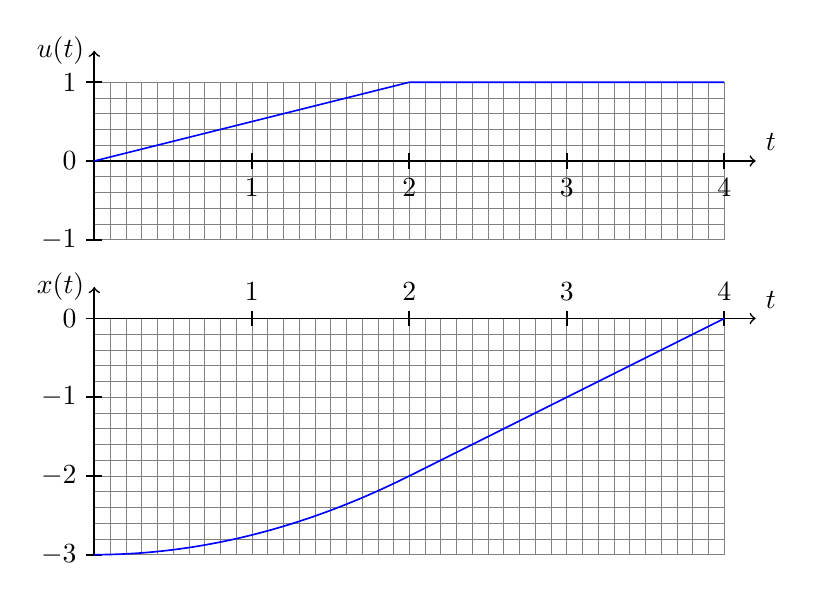
\begin{tikzpicture}[xscale=2]
	\draw[very thin,gray,xstep=1mm,ystep=2mm] (0,-1) grid (4,1);				% сетка
	\draw[semithick,->] (0,0) -- (4.2,0) node[above right] {$t$};				% ось абсцисс
	\draw[semithick,->] (0,-1) -- (0,1.4) node[anchor=east] {$u(t)$};		% ось ординат
	\foreach \t in {1,2,3,4}
		\draw[semithick] (\t cm,1mm) -- (\t cm,-1mm) node[anchor=north] {$\t$};
	\foreach \u in {-1,0,1}
		\draw[semithick] (0.5mm,\u cm) -- (-0.5mm,\u cm) node[anchor=east] {$\u$};
	\draw[semithick,blue] (0,0) -- (2,1) -- (4,1);
	\begin{scope}[yshift=-2cm]
		\draw[very thin,gray,xstep=1mm,ystep=2mm] (0,-3) grid (4,0);			% сетка
		\draw[semithick,->] (0,0) -- (4.2,0) node[above right] {$t$};			% ось абсцисс
		\draw[semithick,->] (0,-3) -- (0,0.4) node[anchor=east] {$x(t)$};	% ось ординат
		\foreach \t in {1,2,3,4}
			\draw[semithick] (\t cm,1mm) -- (\t cm,-1mm) node[above=2mm] {$\t$};
		\foreach \x in {-3,-2,-1,0}
			\draw[semithick] (0.5mm,\x cm) -- (-0.5mm,\x cm) node[anchor=east] {$\x$};
		\draw[semithick,blue,smooth,samples=100,domain=0:2,variable=\t]
			plot( \t, {(\t^2)/4-3} ) -- (4,0);
	\end{scope}
\end{tikzpicture}
\footnotesize \caption{Решение задачи, рассмотренной в первом примере\label{fig:maximum:first_example}}
\end{figure}

\begin{problem}
\[ T\dot{x} + x = Ku \enskip \Rightarrow \enskip \dot{x} = ax + bu \]
\[ \min \, \int\limits_{t_0}^{t_\textit{к}} \bigl( qx^2 + ru^2 \bigr) \, dt, \quad |u| \le U_{ \max } \]
\begin{enumerate}
\item ${{H}^{*}}=-\left( q{{x}^{2}}+r{{u}^{2}} \right)+\psi \left( ax+bu \right)$
\item $\frac{\partial {{H}^{*}}}{\partial u}=-2ru+\psi b=0 $
\[ \left\{ \begin{darray}{l@{\quad}l}
	u = \frac{b}{2r}\psi & \text{при} \left| \frac{b}{2r}\psi \right| \le U_{ \max } \\
	u = U_{ \max } & \text{при} \left| \frac{b}{2r}\psi \right| \ge U_{ \max } 
\end{darray} \right. \]
\item $ \dot{ \psi } = -\frac{\partial H}{\partial x} = 2qx - a\psi , \quad \dot{x} = ax + b\frac{b}{2r}\psi $
\[ \psi = \frac{-a-\sqrt{a^2+b^2q/r}}{b^2} \cdot 2rx \] 
\item $ U_\textit{опт} (t) = \left\{ \begin{darray}{l@{\quad}l}
	\underbrace{ \frac{-a-\sqrt{a^2+b^2q/r}}{b} }_{K_\textit{опт}} x & \text{при} \left| K_\textit{опт} x \right| \le U_{ \max } \\
	\pm U_{ \max } & \text{при} \left| K_\textit{опт} x \right| \ge U_{ \max }
\end{darray} \right. $
\end{enumerate}
\end{problem}

Наибольшее применение принцип максимума нашёл при минимизации времени переходного процесса (максимизации быстродействия), так как в этом случае $ \underset{ u \in U }{ \min } \=, J = \int\limits_{t_0}^{t_\textit{к}} F(x,u) \, dt = \int\limits_{t_0}^{t_\textit{к}} 1 \, dt = t_\textit{к} - t_0 $ имеет простейшую подынтегральную функцию и гамильтониан $ H^* = -1 + \sum\limits_{i=1}^{n} \psi _i (t) \Phi _i (x,u) = -1 + \psi ^T (Ax+Bu) $, от управления зависит только последнее слагаемое и в условиях ограничений на управление  
$\left| u \right|\le {{U}_{m}}$ решение имеет естественный вид: $ u = U_m \cdot sign( \psi ^T B ) $, т.\=,е. оптимальная система является релейной с определением переключения по знаку вспомогательной функции $ B^T \psi $, где $ \dot{ \psi } = -A^T\psi \enskip \Rightarrow \enskip \psi (t) = -e^{-A^Tt} \psi (0) $, однако, поиск $ \psi (0) $ приводит либо к системе трансцендентных уравнений, трудно решаемых в общем виде, либо к итерационному поиску.

В простейшем случае, когда объект представим последовательным соединением двух интеграторов:
\[ \ddot{x} = u, \quad  |u| \le U_m \]
\vspace{-1.5\baselineskip}
\begin{figure*}[ht] \centering
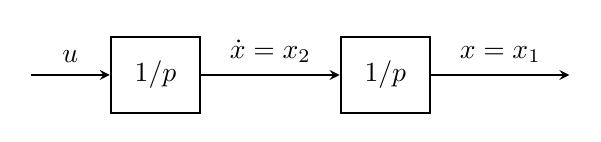
\begin{tikzpicture}	
	[	auto,
		block/.style={rectangle,draw=black,thick,inner sep=2ex},
		vec/.style={->,>=stealth,semithick,inner sep=1ex},
		point/.style={inner sep = 0pt}	]
	\node[block] (int1) {$ 1/p $};
	\node[block] (int2) [right = 5em of int1] {$ 1/p $};
	\draw[vec] (int1) to node{$ \dot{x} = x_2 $} (int2);
	\node[point] (input) [left = of int1] {};
	\draw[vec] (input) to node{$u$} (int1);
	\node[point] (output) [right = 5em of int2] {};
	\draw[vec] (int2) to node{$ x = x_1 $} (output);
\end{tikzpicture}
\end{figure*}
\[ \left| \begin{matrix}
	\dot{x}_1 \\
	\dot{x}_2
\end{matrix} \right| = \left| \begin{matrix}
   0 & 1  \\
   0 & 0  
\end{matrix} \right| \cdot \left| \begin{matrix}
   {{x}_{1}}  \\
   {{x}_{2}} 
\end{matrix} \right| + \left| \begin{matrix}
   0  \\
   1  
\end{matrix} \right| u \]
Гамильтониан $H\left( \psi ,x,u \right)=-1+{{\psi }_{1}}{{x}_{2}}+{{\psi }_{2}}u$ и $max$ достигается при $ u_\textit{опт} (t) = U_m \cdot sign \=, \psi _2 $, где $ \dot{ \psi }_2 = -\frac{\partial H}{\partial x_2} = \psi _1, \enskip \dot{\psi }_1 = -\frac{\partial H}{\partial x_1} = 0 $ и $ \psi _2 (t) = C_1t + C_2 $, произвольные постоянные, при любом наборе которых $ \psi _2 $ может иметь только два интервала с разными знаками, соответственно $ u_\textit{опт} (t) $ --- кусочно-постоянная функция, принимающая значения $ +U_m $ и $ -U_m $. Отсюда, для перевода из нулевого начального состояния в заданное конечное (например, положительное $ x (t_\textit{к}) > 0 $) будем иметь два интервала: разгон и торможение, и переключение произойдёт ровно посередине. Если будет ограничена скорость набора $ |x_2| \le x_{2m} $, то в интервале $ t_1 \to t_2 $ потребуется обнулить управление и увеличится время переходного процесса $ t'_\textit{к} > t_\textit{к} $, а управление будет иметь три интервала: $ +U_m $, $ 0 $, $ -U_m $.
\[ u_\textit{опт}^{\textit{огр.}x_2} (t) = \left\{ \begin{darray}{l@{\quad}l}
	0 & \text{при} \bigl| \psi _2 \bigr| \le 1  \\
	sign \=, \psi _2 & \text{при} \bigl| \psi _2 \bigr| > 1
\end{darray} \right. \]

	\subsection{Синтез оптимального по быстродействию управления для линейных систем\label{maximum:fastest}}
В общем случае задача синтеза оптимального по быстродействию управления линейным объектом
\[ \dot{X} = \Phi (x,u) = Ax + Bu, \quad \min \int\limits_{t_0}^{t_\textit{к}} 1 \=, dt = t_\textit{к} - t_0 \]
с возможными ограничениями на $ \bigl| x_i \bigr| \le X_i $ осуществляется с помощью принципа максимума на основе составления функции Гамильтона:
\[ H( \psi , x, u ) = -1 + \psi ^T (AX+Bu) \]
\[ u_\textit{опт} = U_{ \max } \cdot sign \left( \frac{\partial H}{\partial u} \right) = U_{ \max } \cdot sign \left( B^T \psi \right) \]
\[ \dot{ \psi } (t) = - \psi ^T (t) \frac{\partial \Phi (x,u)}{\partial x} = - \psi ^T (t) A = -A^T \psi (t) \enskip \Rightarrow \enskip \psi (t) = e^{-A^Tt} \cdot \psi (0) \]
Это набор экспонент, поиск которых в общем виде затруднён. Однако, в частных случаях был получен ряд важных результатов.
\begin{enumerate}
\item Если собственные числа матрицы $A$ --- различные вещественные, то сумма $n$ экспонент $ B^T \psi $ может пересекать ось абсцисс и менять знак только $ (n-1) $ раз. Фельдбаум~А.\=,А. доказал теорему об $n$ интервалах:
\begin{theorem}
Если объект управления описывается ЛДУ $n$-го порядка с постоянными коэффициентами и корни его характеристического уравнения вещественные отрицательные или нулевые, то для оптимального управления по $t$ необходимо и достаточно не более $n$ интервалов максимального по значению управления $ U_m $, а знаки чередуются не более $ (n-1) $ раз.
\end{theorem}
\item Оптимальное управление для линейных систем с комплексными полюсами не удовлетворяет теореме Фельдбаума, число переключений управления не связано с порядком системы, а зависит от её начального состояния.
\item Наличие только ограниченного числа вариантов управляющего сигнала $ \pm U_m $ позволяет разделить всё фазовое пространство СУ на области с помощью гиперповерхностей $ S(x) = 0 $, в каждой из которых управление постоянно. Такой подход называется методом фазового пространства, и позволяет вычислять управление на основе анализа нелинейных зависимостей: $ u_\textit{опт} = -U_{ \max } \cdot sign \bigl[ S(x) \bigr] $.
\end{enumerate}

\vspace{-\baselineskip}
\begin{problem}
\[ \ddot{x} = u(t), \qquad \left| \begin{matrix}
   \dot{x}_1  \\
   \dot{x}_2
\end{matrix} \right| = \left| \begin{matrix}
   0 & 1  \\
   0 & 0
\end{matrix} \right| \cdot \left| \begin{matrix}
   x_1  \\
   x_2
\end{matrix} \right| + \left| \begin{matrix}
   0  \\
   1
\end{matrix} \right| u, \qquad \left\{ \begin{darray}{l}
	\dot{x}_1 = x_2 \\
	\dot{x}_2 = u
\end{darray} \right. \]
\[ \frac{dx_1}{dt} \!\! \biggm/ \!\! \frac{dx_2}{dt} = \frac{x_2}{u} \enskip \Rightarrow \enskip \frac{dx_1}{dx_2} = \frac{x_2}{u} \enskip \Rightarrow \enskip u \=, dx_1 = x_2 \=, dx_2 \]
\[ \begin{darray}{l@{\quad}l@{\quad}l}
	u = + U_m & \Rightarrow & U_m x_1 = \frac{x_2^2}{2} \\
	u = - U_m & \Rightarrow & - U_m x_1 = \frac{x_2^2}{2}
\end{darray} \]
Откуда получаем траектории следующего вида:
\begin{center}
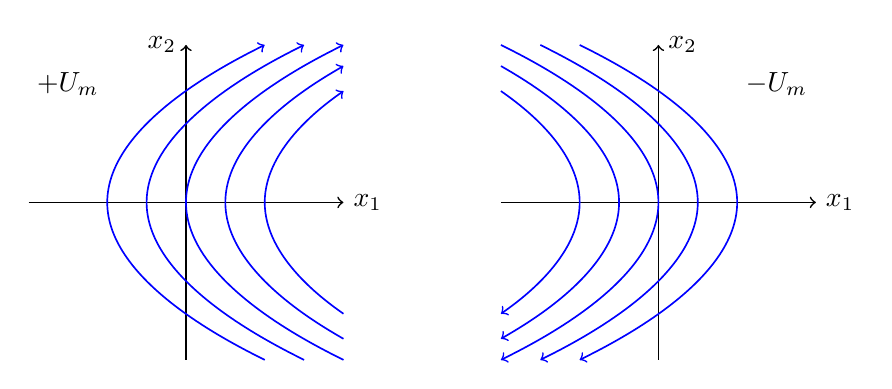
\begin{tikzpicture}
	\draw[semithick,->] (-2,0) -- (2,0) node[right] {$ x_1 $};
	\draw[semithick,->] (0,-2) -- (0,2) node[left] {$ x_2 $};	
	\begin{scope}[semithick,blue,<-,rotate=-90]
		\foreach \c in {-1,-0.5,0}
			\draw (-2,2+\c) parabola bend (0,0+\c) (2,2+\c);
		\draw (-3^0.5,2) parabola bend (0,0.5) (3^0.5,2);
		\draw (-2^0.5,2) parabola bend (0,1) (2^0.5,2);
	\end{scope}
	\node at (-1.5,1.5) {$ +U_m $};
	\begin{scope}[xshift=6cm]
		\draw[semithick,->] (-2,0) -- (2,0) node[right] {$ x_1 $};
		\draw[semithick,->] (0,-2) -- (0,2) node[right] {$ x_2 $};
		\begin{scope}[semithick,blue,<-,rotate=90]
			\foreach \c in {-1,-0.5,0}
				\draw (-2,2+\c) parabola bend (0,0+\c) (2,2+\c);
			\draw (-3^0.5,2) parabola bend (0,0.5) (3^0.5,2);
			\draw (-2^0.5,2) parabola bend (0,1) (2^0.5,2);
		\end{scope}
		\node at (1.5,1.5) {$ -U_m $};
	\end{scope}
\end{tikzpicture}
\end{center}

Выделим линию:
\[ S \bigl( x_1, x_2 \bigr) = x_1 + sign \bigl( x_2 \bigr) \frac{x_2^2}{2U_m} = x_1 + \frac{x_2 \cdot \bigl| x_2 \bigr| }{2U_m} = 0 \]
\[ u = -U_m \cdot sign \Bigl( S \bigl( x_1, x_2 \bigr) \Bigr) \]
Тогда получим фазовые траектории в виде:
\begin{center}
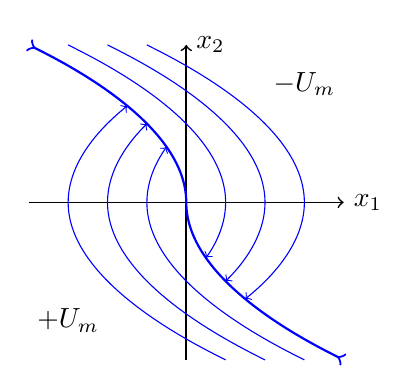
\begin{tikzpicture}
	\draw[semithick,->] (-2,0) -- (2,0) node[right] {$ x_1 $};
	\draw[semithick,->] (0,-2) -- (0,2) node[right] {$ x_2 $};	
	\begin{scope}[blue,rotate=90]
		\path[name path=superline,thick,draw,>-<] (-2,-2) parabola bend (0,0) (0,0) parabola (2,2);
		\foreach \c in {-1.5,-1,-0.5} {
			\path[name path=line one] (2,2+\c) parabola bend (0,0+\c) (-2,2+\c);
			\draw[name intersections={of=superline and line one},->]
				(2,2+\c) parabola bend (0,0+\c) (intersection-1);
		}
		\foreach \c in {0.5,1,1.5} {
			\path[name path=line one] (-2,-2+\c) parabola bend (0,0+\c) (2,-2+\c);
			\draw[name intersections={of=superline and line one},->]
				(-2,-2+\c) parabola bend (0,0+\c) (intersection-1);
		}
	\end{scope}
	\node at (1.5,1.5) {$ -U_m $};
	\node at (-1.5,-1.5) {$ +U_m $};
\end{tikzpicture}
\end{center}
\end{problem}
Аналитические представления для поверхностей переключения как функций координат полностью разрешимы для линейных систем второго порядка. Для большего порядка решения найдены только в частных случаях.

 \begin{enumerate}[resume]
 \item При построении оптимального управления реальными объектами существует как минимум три причины невозможности его технической реализации:
 \begin{itemize}
 \item неидеальность (неточность) математической модели объекта управления;
 \item упрощения, принимаемые при реализации закона (алгоритма) объекта управления;
 \item неточность (непостоянство) характеристик реальных элементов, реализующих управление (гистерезис, зона нечувствительности и~т.\=,п.).
  \end{itemize}

Поэтому на практике реализуются квазиоптимальные или субоптимальные системы, использующие скользящие режимы движения. Реализация устройства управления в этом случае не требует нелинейных операций, используются только линейные усилители (с различными коэффициентами усиления) и релейные переключатели.
 \end{enumerate}
 
	\subsection{Уравнение Риккати для синтеза оптимальных систем\label{maximum:Riccati}}
Для линейных объектов управления $\dot{x}=Ax+Bu$ и минимизируемого квадратичного функционала $J=\frac{1}{2}\int\limits_{t_0}^{t_\textit{к}} \bigl( x^TQx + u^TRu \bigr) \=, dt$ без учёта ограничений $u_\textit{опт} (t) = K_\textit{ос}x$.

Функция Гамильтона:
\[ H^* = -\frac{1}{2}x^TQx - \frac{1}{2}u^TRu + \psi ^T (Ax+Bu) \]
\[ \frac{\partial H^*}{\partial u} \Big| _{u=u_\textit{опт}} = 0 \]
\[ \frac{\partial H^*}{\partial u} = -Ru_\textit{опт}(t) + \psi ^TB = -Ru_\textit{опт} + B^T\psi = 0 \]
\[ u_\textit{опт}(t) = R^{-1}B^T\psi \]

При этом обеспечивается максимум $ H^* $, т.\=,к.
\[ \frac{\partial ^2 H^*}{\partial u^2} \Big| _{u=u_\textit{опт}} = -R < 0 \]

Запишем канонические уравнения:
\[ \left\{ \begin{darray}{l}
   \dot{x} = Ax+BR^{-1}B^T\psi \\
   \dot{ \psi } = Qx - \psi ^T A = Qx - A^T \psi
\end{darray} \right. \]

Сравнивая $u_\textit{опт} = K_\textit{ос}x$ и $u_\textit{опт} = R^{-1}B^T\psi $, можно ввести $ \psi = -P(t)x $, дифференцируя которое, получим $ \dot{ \psi } = -\dot{P}(t)x - P(t)\dot{x} $, тогда:
\[ \left\{ \begin{darray}{l}
   \dot{x} = Ax - B R^{-1} B^T P(t)x \\
   \dot{ \psi } = Qx + A^T P(t)x
\end{darray} \right. \]
\[ -\dot{P}(t)x - P(t)\bigl( Ax - BR^{-1}B^TP(t)x \bigr) = Qx + A^TP(t)x \]
\begin{equation}
\dot{P}(t) + A^TP(t) + P(t)A - P(t)BR^{-1}B^TP(t) = Q
\end{equation}

Это дифференциальное уравнение Риккати, после решения которого можно получить:
\[ u_\textit{опт}(x) = -R^{-1}B^TP(t)x(t) \]

Для объектов с постоянными по времени параметрами $ \dot{P}(t) = 0 $ и при $ t_\textit{к} \to \infty $ $ P(t) = \overline{P} $ --- определённо положительная симметричная матрица коэффициентов. В случае ограничений типа $ \bigl| u(t) \bigr| \le U_m $ получим нелинейный закон с насыщением, аналогичный простейшему случаю.

\clearpage   
\section{Динамическое программирование\label{dyn_prog}}
	\subsection{Определение\label{dyn_prog:def}}
В технике и экономике существует класс объектов и процессов, управление которыми осуществляется на основе ограниченного числа решений, принимаемых последовательно в некоторые фиксированные моменты времени. Определение закона (алгоритма) управления для таких объектов связано с решением задачи по методу многошагового выбора, который был предложен американским учёным Р.~Беллманом и назван \textit{динамическим программированием}.

В основу положен принцип оптимальности, согласно которому оптимальное управление определяется конечной целью и состоянием системы в данный момент времени независимо от предыстории.

Задачей оптимизации считается определение оптимальных управлений $ u^\textit{о}(t) $ и траекторий $ x^\textit{о}(t) $ из условия минимума функционала $ J = \int\limits_{t_0}^{t_\textit{к}} F(x,u,t) \=, dt $ при заданных уравнениях объекта $ \dot{x} = \Phi (x,u) = Ax+Bu $ и граничных значениях $ x(t_0), \enskip x(t_\textit{к}), \enskip t_0 \le t \le t_\textit{к} $, а также допустимых интервалах для $ x(t) \in X, \enskip u(t) \in U $.

В методе динамического программирования вводится вспомогательная функция Беллмана:
\begin{equation}
S(t,x) = \underset{u \in U}{ \min } \=, \int\limits_{t_0}^{T} F(x,u,t) \=, dt
\end{equation}

В соответствии со сформулированным принципом минимум функционала зависит только от момента времени, значения $x$ в этот момент и конечного момента. Тогда для любого промежуточного момента $ t \in t_0 + \Delta t < T $ выполнено равенство
\[ S \bigl( t_0 + \Delta t, T, x_{\Delta t} \bigr) = \underset{u \in U}{ \min } \=, \int\limits_{t_0 + \Delta t}^{T} F(x,u,t) \=, dt, \]
где $ x_{ \Delta t } = x \bigl( t_0 \bigr) + \Delta x $.

\begin{multline*}
S(t,x) = \underset{u \in U}{ \min } \=, \left[ \int\limits_{t_0}^{t_0 + \Delta t} F(x,u,t) \=, dt + \int\limits_{t_0 + \Delta t}^{T} F(x,u,t) \=, dt \right] = \\* \underset{u \in U}{ \min } \=, \left[ \int\limits_{t_0}^{t_0 + \Delta t} F(x,u,t) \=, dt + S \bigl( t_0 + \Delta t, T, x_{\Delta t} \bigr) \right]
\end{multline*}

Это выражение должно использоваться для определения оптимальных управлений на интервале $ \bigl[ t_0, t_0 + \Delta t \bigr] $. При решении либо решают функциональные уравнения Беллмана в частных производных, либо применяют численные методы.

	\subsection{Функциональное уравнение Беллмана для синтеза оптимального управления\label{dyn_prog:Bellman_equation}}
Первое слагаемое с точностью до малых более высокого порядка, чем $ \Delta t $, можно приблизительно записать так:
\[ \int\limits_{t_0}^{t_0 + \Delta t} F(x,u,t) \=, dt \approx F(x,u,t) \Delta t = \Delta J \]

Второе слагаемое, определяющее значение $ S\left( t+\Delta t,x+\Delta x \right)$ для любого $t+\Delta t$ разложим в ряд Тейлора. Ограничиваясь линейными членами относительно $ \Delta x_i $ и $ \Delta t $ и переходя к пределу (если функция $ S(t,x) $ имеет непрерывные частные производные по всем $ x_i (t) $ и $t$), запишем:
\begin{multline*}
S \left( t+\Delta t,x+\Delta x \right)=S\left( t,x \right)+\sum\limits_{i=1}^{n}{\frac{\partial S}{\partial {{x}_{i}}}}\cdot \Delta {{x}_{i}}+\frac{\partial S}{\partial t}\Delta t = \\ S\left( t,x \right)+\left[ \sum\limits_{i=1}^{n}{\frac{\partial S}{\partial {{x}_{i}}}}\cdot \frac{d{{x}_{i}}}{dt}+\frac{\partial S}{\partial t} \right]\Delta t
\end{multline*}
Тогда можем записать:
\[ S\left( t,x \right)=\underset{u\in U}{\mathop{\min }}\,\left\{ F\left( x,u,t \right)\Delta t+S\left( t,x \right)+\left[ \sum\limits_{i=1}^{n}{\frac{\partial S}{\partial {{x}_{i}}}\cdot {{{\dot{x}}}_{i}}+\frac{\partial S}{\partial t}} \right]\Delta t \right\} \]

Откуда, переходя к пределу при $ \Delta t \to 0 $, получим нелинейное дифференциальное уравнение Беллмана в частных производных относительно неизвестной функции $S\left( t,x \right)$:
\begin{equation}\label{equ:dyn_prog:Bellman}
\underset{u\in U}{\mathop{\min }}\,\left\{ F\left( x,u,t \right)+\left[ \sum\limits_{i=1}^{n}{\frac{\partial S}{\partial {{x}_{i}}}\cdot {{\varphi }_{i}}\left( x,u,t \right)+\frac{\partial S}{\partial t}} \right] \right\}=0
\end{equation}

Необычность этого уравнения в том, что оно содержит операцию минимизации. Регулярных аналитических методов решения таких уравнений нет. Однако, Лётов~А.\=,М. предложил методику поиска $ u^\textit{о} (t) = u \left( \frac{ \partial S(x,t) }{ \partial x } \right) $, \vspace{0.5ex} тогда уравнение \eqref{equ:dyn_prog:Bellman} становится обычным уравнением в частных производных:
\[ F(x,u,t) + grad_{x}^{T} \=, S(x,t) \cdot \Phi (x,u) + \frac{ \partial S(x,t) }{ \partial t } = 0 \]
с граничным условием $ S \bigl( x^\textit{о}, T \bigr) = 0 $.

Если $ S(x) $ не зависит явным образом от $t$, то $\frac{\partial S}{\partial t}=0$ и поиск оптимального управления можно производить по уравнению:
\[ \frac{ \partial F(x,u,t) }{ \partial u_j } + \sum\limits_{i=1}^{n}{\frac{\partial S}{\partial {{x}_{i}}}\frac{\partial {{\varphi }_{i}}}{\partial {{u}_{j}}}} = 0 \]

Такой подход наиболее подходит, когда ищется решение для линейно\-/квадратичных задач и вспомогательная функция берётся в виде квадратичной формы $ S(x) = \sum\limits_{i,j=1}^{n} A_{ij} x_i x_j $.

\begin{problem}
\[ T \dot{x} + x = Ku \enskip \Rightarrow \enskip \dot{x} = ax + bu \]
\[ \min \int\limits_{0}^{ \infty } \bigl( qx^2 + ru^2 \bigr) \=, dt, \qquad S(x) = Ax^2 \]
Тогда функциональное уравнение Беллмана запишется в виде:
\[ qx^2 + ru^2 + (ax+bu) \cdot \frac{\partial S}{\partial x} = 0 \]
\[ 2ru + b\frac{\partial S}{\partial x} = 0 \enskip \Rightarrow \enskip u^\textit{о} (t) = - \frac{b}{2r} \frac{\partial S}{\partial x} = \underbrace{-\frac{b}{r}A}_{K_\textit{ос}} x(t) \]
Для нахождения $A$ и $ K_\textit{ос} $:
\[ qx^2 + r{ \left( -\frac{b}{r}Ax \right) }^2 + \biggl( ax + b\Bigl( -\frac{b}{r}Ax \Bigr) \biggr) Ax = 0 \]
Возведя в квадрат, вынеся $x$ и сгруппировав, получим:
\[ b^2 A^2 - 2arA - qr = 0 \]
\[ A = \frac{ r \left( a \pm \sqrt{ a^2 + b^2 q/r } \right) }{ b^2 } \qquad (A>0) \]
\[ K_\textit{ос} = -\frac{b}{r}A = \frac{ -a - \sqrt{ a^2 + b^2 q/r } }{b} \]
\end{problem}

Подводя итог, применение метода для задачи в форме Лагранжа можно сформулировать в виде алгоритмической процедуры:
\begin{enumerate}
\item составить функцию Беллмана
\[ B \left( t, x, u, \frac{ \partial S(x,t) }{ \partial x } \right) = F(x,u,t) + grad_{x}^{T} \=, S(x,t) \cdot \Phi (x,u,t) \]
\item минимизировать функцию Беллмана по $ u \in U $
\[ \underset{ u \in U }{ \min } \=, B \left( t, x, u, \frac{ \partial S }{ \partial x } \right) = B^* \left( t, x, \frac{\partial S}{\partial x} \right) , \]
определяя управление, как явную функцию $ x $ и $ \frac{\partial S}{\partial x} $
\[ u^* = u \left( x^*, \frac{\partial S}{\partial x} \right) \]
\item составить уравнение Беллмана
\[ B^* \left( t, x, \frac{\partial S}{\partial x} \right) + \frac{ \partial S \bigl( x^*, t \bigr) }{\partial t} = 0, \quad S \bigl( x^*, T \bigr) = 0 \]
\item решением этого уравнения является функция $ S(x,t) $, по которой определяются  $ \frac{\partial S}{\partial x} $, а затем искомое оптимальное управление  $ u^* = u \left( x^*, \frac{\partial S}{\partial x} \right)$.
\end{enumerate}

\begin{problem}

Применим эту процедуру для управляемого объекта:
\[ \dot{x} = Ax + bu, \quad x(0) = x_0 \]
\[ \underset{u}{ \min } \=, J(x,u) = \int\limits_{0}^{T} \bigl( x^2 + cu^2 \bigr) \=, dt \]

Это задача Лагранжа с фиксированным временем и подвижным правым концом. При этом естественно искать решение в классе линейных функций $ u(t) = K(t) \cdot x(t) $.

\begin{enumerate}
\item Составим функцию Беллмана
\[ B = x^2 + cu^2 + \frac{\partial S(x,t)}{\partial x} (ax+bu) \]
\item Найдём её минимум
\[ \frac{\partial B}{\partial u} = 2cu(t) + b\frac{\partial S(x,t)}{\partial x} = 0 \enskip \Rightarrow \enskip u^* = -\frac{b}{2c} \frac{\partial S(x,t)}{\partial x} \]
\[ \frac{ \partial ^2 B }{ \partial u^2 } = 2c > 0 \enskip \Rightarrow \enskip \text{достаточность выполнена} \]
\item Составим дифференциальное уравнение Беллмана, подставляя $ u^* $ вместо $ u $
\[ x^2 - \frac{b^2}{c} { \left( \frac{\partial S}{\partial x} \right) }^2 \left( \frac{1}{4} - \frac{1}{2} \right) + ax \frac{\partial S}{\partial x} + \frac{\partial S}{\partial t} = 0, \quad S \bigl( x(T), T \bigr) = 0 \] 
\end{enumerate}

Это нелинейное уравнение первого порядка в частных производных, в общем случае с труднонаходимым решением. Однако, если решение ищется как линейное, то $ S(t) = p(t) x^2 $. Составим уравнение относительно новой неизвестной $ p(t) $:
\[ \frac{\partial S}{\partial x} = 2p(t) \cdot x, \quad u^* = -\frac{b}{c} p(t) \cdot x \]
\[ x^2 \left( \dot{p}(t) - \frac{b^2}{4c^2} \cdot 4p^2(t) - 2ap(t) + 1 \right) = 0, \quad p(T) = 0 \]

В скобках нелинейное дифференциальное уравнение первого порядка типа Риккати с граничным условием на правом конце. Это уравнение можно решить методом разделения переменных, и решение принимает вид:
\[ p(t) = p_1 p_2 \frac{ 1 - \exp \left( -\frac{b^2}{c^2} \cdot \bigl( p_1 - p_2 \bigr) (T-t) \right) }{ p_2 - p_1 \exp \left( -\frac{b^2}{c^2} \cdot \bigl( p_1 - p_2 \bigr) (T-t) \right) } , \]
где $ p_1 $, $ p_2 $ --- корни уравнения $ \frac{b^2}{c^2} p^2 (t) + 2ap(t) - 1 = 0 $. Если $ T \to \infty $, то $ p(t) = \max \bigl( p_1, p_2 \bigr) $.

\end{problem}

Рассмотрим задачу Лагранжа с закреплёнными концами и свободным временем для произвольной динамической системы:
\[ \dot{x} = \Phi (x,u), \quad x(0) = x_0, \quad x(T) = x_\textit{к}, \quad u \in U \]

Следует найти допустимое управление, переводящее эту систему из $ x_0 $ в $ x_\textit{к} $ так, чтобы критерий качества $ J(x,u,T) = \int\limits_{0}^{T} F(x,u) \=, dt $ принимал наименьшее значение. Для решения этой задачи согласно процедуре метода введём функцию $ R(x) $, которая совпадает с наименьшим значением критерия вдоль оптимальной траектории. Эта функция зависит только от текущего состояния. Уравнение Беллмана в этом случае принимает вид:
\[ \underset{u \in U}{ \min } \=, \Bigl[ F \bigl( x(t), u(t) \bigr) +grad_{x}^{T} R(x) \Phi \bigl( x(t), u(t) \bigr) \Bigr] = 0 \]

Задача максимального быстродействия является частным случаем сформулированной задачи Лагранжа с закреплёнными концами и свободным временем, если положить в ней $ F(x,u) \equiv 1 $. Содержательный смысл функции $ R(x) $ --- наименьшее время перевода системы из текущего состояния $ x(t) $ до цели $ x_\textit{к} $. Уравнение Беллмана для этой задачи принимает вид:
\[ \underset{ u(t) \in U }{ \min } \=, \Bigl[ grad_{x}^{T} R(x) \cdot \Phi (x,u) \Bigr] = -1, \quad R \bigl( x_\textit{к} \bigr) = 0 \]

Уравнение Беллмана имеет простую геометрическую интерпретацию: пусть конечной целью является начало координат, тогда $ R(x) = T^* $ --- множество точек фазового пространства, для которых время перехода составляет ровно $ T^* $. Эту гиперповерхность называют \textit{изохроной}.

Записав уравнение Беллмана в форме максимизации (т.\=,е.~поменяв знак): $ \underset{u \in U}{ \max }\=, \Bigl[ \bigl( -grad_{x}^{T} R(x) \bigr) \Phi (x,u) \Bigr] = 1 $, получим геометрическое условие оптимальности в задаче быстродействия:

\textit{Оптимальное управление следует выбирать таким, чтобы в любой точке изохроны вектор нормали $ -grad \=, R(x) $ и текущий вектор фазовой скорости $ \dot{x} = \Phi (x,u) $ были предельно близки, и, если управление не ограничено, то оба вектора имеют одно направление.}

\begin{problem}
Найти допустимое управление $ \bigl| u(t) \bigr| \le 1 $ для быстрейшего перевода из произвольной точки фазового пространства в начало координат системы:
\[ \dot{x}_1 = x_2, \quad \dot{x}_2 = u, \quad x_1(0) = x_0 \]
 
\begin{enumerate}
\item Составим функциональное соотношение Беллмана:
\[ \underset{ |u| \le 1}{ \min } \=, \left[ \frac{\partial R}{\partial x_1} \cdot x_2 + \frac{\partial R}{\partial x_2} \cdot u \right] = -1, \quad R(0) = 0 \] 
\item Минимум выражения в скобках достигается при 
\[ u^* = -sign \left( \frac{\partial R}{\partial x_2} \right) \]
\item Дифференциальное уравнение Беллмана принимает вид: 
\[ 1 + \frac{\partial R}{\partial x_1} \cdot x_2 - \left| \frac{\partial R}{\partial x_2} \right| = 0, \quad R(0) = 0 \]
\item Для решения этого уравнения рассмотрим варианты:
\begin{itemize}
\item Область \textbf{1} $ \left\{ \left( \begin{matrix}
	x_1 \\
	x_2
\end{matrix} \right) \=, : \enskip \frac{\partial R}{\partial x_2} > 0 \right\} \enskip \Rightarrow \enskip u^* = -1 \enskip \Rightarrow \enskip $ уравнение Беллмана принимает вид: 
\[ 1 + \frac{\partial R}{\partial x_1} x_2 - \frac{\partial R}{\partial x_2} = 0 \enskip \Rightarrow \enskip R_1 = x_2 + 2\sqrt{ \frac{x_2^2}{2} + x_1 } \]
\item Область \textbf{2} $ \left\{ \left( \begin{matrix}
	x_1 \\
	x_2
\end{matrix} \right) \=, : \enskip \frac{\partial R}{\partial x_2} < 0 \right\} \enskip \Rightarrow \enskip u^* = 1 \enskip \Rightarrow \enskip $ уравнение Беллмана принимает вид:
\[ 1 + \frac{\partial R}{\partial x_1} x_2 + \frac{\partial R}{\partial x_2} = 0 \enskip \Rightarrow \enskip R_2 = -x_2 + 2\sqrt{ \frac{x_2^2}{2} - x_1 } \]
\end{itemize}
\end{enumerate}

Границей между областями \textbf{1} и \textbf{2} будет кривая:
\[ x_1 + \frac{ x_2^2 \cdot sign(x_2) }{2} = 0 \]

А найденное оптимальное управление
\[ u^* = -sign \left( x_1 + \frac{ x_2^2 \cdot sign(x_2) }{2} \right) \]
имеет явную зависимость от фазовых координат, что позволяет синтезировать замкнутую структуру управления.

Отметим один замечательный результат. В каждой области можно выделить аналитическое выражение для  семейства изохрон уровня $ T^* $:
\begin{itemize}
\item в первой:
\[ x_1 + \frac{x_2^2}{2} - \frac{ { \bigl( T^* - x_2 \bigr) }^2 }{4} = 0 \]
\item во второй:
\[ x_1 - \frac{x_2^2}{2} + \frac{ { \bigl( T^* + x_2 \bigr) }^2 }{4} = 0 \]
\end{itemize}

А на границе:
\[ x_1 + \frac{ x_2 \cdot T^* }{2} = 0 \]

Таким образом, можно изобразить семейство изохрон, и для любой точки, например, $ \left( \begin{matrix} x_1 \\ x_2 \end{matrix} \right) = \left( \begin{matrix} 4 \\ 0 \end{matrix} \right) $ изобразить вектор $ grad \=, R = \left( \begin{matrix} 0.5 \\ 1 \end{matrix} \right) $ и вектор фазовой скорости $ \Phi (x,u) = \left( \begin{matrix} 0 \\ u \end{matrix} \right) $. Из всех возможных управлений лишь при $ u = -1 $ будет наибольшая проекция на направление антиградиента к изохроне в этой точке. Значит, оптимальное управление $ u^* \left( \begin{matrix} 4 \\ 0 \end{matrix} \right) = -1 $.

\end{problem}

	\subsection{Численное решение уравнений динамического программирования\label{dyn_prog:numerical}}

Уравнение минимизации
\[ \underset{u \in U}{ \min } \=, \left\{ F(x,u,t) + \sum\limits_{i=1}^{n} \frac{\partial s}{\partial x_i} \cdot \varphi _i (x,u,t) + \frac{\partial s}{\partial t} \right\} = 0 \]
или соответствующие ему функциональные уравнения в частных производных
\[ \left\{ \begin{darray}{l}
	F(x,u,t) + \sum\limits_{i=1}^{n} \frac{\partial s}{\partial x_i} \cdot \varphi _i (x,u,t) + \frac{\partial s}{\partial t} = 0 \\
	\frac{\partial F}{\partial u_j} + \sum\limits_{i=1}^{n} \frac{\partial s}{\partial x_i} \cdot \frac{\partial \varphi _i}{\partial u_j} = 0, \quad j = \overline{1,r} \end{darray} \right. \]
далеко не всегда удаётся решить аналитически. Поэтому применяется численный подход в виде многошагового процесса, являющегося приближенным. Для этого исходные уравнения объекта заменяют конечно\-/разностными:
\[ \left\{ \begin{darray}{l}
	\Delta x_k = \Phi \bigl( x_{k-1}, u_k \bigr) \Delta t \\
	x_k = x_{k-1} + \Delta x_k, \quad x_0 = x \bigl( t_0 \bigr) , \quad x_N = x(T) \\
	u_k = u_{k-1} + \Delta u_k \\
	\Delta t = \frac{ T - t_0 }{N} ,
\end{darray} \right. \]
где $N$ --- число шагов (принятых расчётных интервалов).

\[ J = \sum_{k=1}^N F_k \bigl( x_{k-1}, u_k \bigr) \Delta t \]

На каждом интервале (шаге) $ u_k $ сохраняет неизменное значение, определённое для его начала. Оптимальное управление можно определить, найдя оптимальные значения для каждого интервала $ u_1^\textit{о}, u_2^\textit{о}, \ldots u_N^\textit{о} $, такие, что $ u_k \in U, \enskip x_k \in X $ и обеспечивается $ \min \=, J $.

При численном решении задачи участки процесса рассматриваются в последовательности обратной их номеру, т.\=,е.~от конца к началу. Рассмотрим начало последнего участка, т.\=,е.~момент времени $ t_{N-1} = (N-1) \Delta t $, ему соответствуют координаты $ x_{N-1} $. Согласно принципу оптимальности необходимо, чтобы было выбрано оптимальное управление на последнем шаге $ u_N^\textit{о} $, переводящее объект из состояния $ x_{N-1} $ в $ x_N $. Выбор $ u_N^\textit{о} $ влияет лишь на последний член суммы в функционале $ J_N = F_N \bigl( x_{N-1}, u_N \bigr) \Delta t $. Выбрав $ u_N^\textit{о} $, обеспечивающее минимум $ J_N $, получим $ s_N \bigl( x_{N-1} \bigr) = \underset{ u^\textit{о} \in U }{ \min } \=, \Bigl[ F_N \bigl( x_{N-1}, u_N^\textit{о} \bigr) \Delta t \Bigr] $.

В результате решения задачи на последнем шаге получены значения $ s_N \bigl( x_{N-1} \bigr), \enskip x_{N-1} \bigl( t_{N-1} \bigr), \enskip u_N^\textit{о} \bigl( x_{N-1} \bigr) $, которые запоминаются. Перейдём к предпоследнему шагу $ (N-2) $, т.\=,е.~моменту времени $ t_{N-2} = (N-2) \Delta t $. Этому интервалу соответствуют координаты $ x_{N-2} $. Теперь нужно выбрать $ u_{N-1}^\textit{о} $ из условия $ \min $ двух последних членов суммы:
\[ J_{N-1} + J_N = F_{N-1} \bigl( x_{N-2}, u_{N-1} \bigr) \Delta t + F_N \bigl( x_{N-1}, u_N^\textit{о} \bigr) \Delta t, \]
с учётом того, что $ u_N^\textit{о} $ уже выбрано. Решая, получим:
\[ s_{N-1} \bigl( x_{N-2} \bigr) = \underset{ u_{N-1}^\textit{о} \in U }{ \min } \=, \Bigl[ F_{N-1} \bigl( x_{N-2}, u_{N-1}^\textit{о} \bigr) \Delta t + s_N \bigl( x_{N-1} \bigr) \Bigr] \]

Так как $ x_{N-1} = x_{N-2} + \Delta x_{N-1} = x_{N-2} + \Phi \bigl( x_{N-2}, u_{N-1}^\textit{о} \bigr) \Delta t $, то можно записать:
\begin{multline*}
s_{N-1} \bigl( x_{N-2} \bigr) = \underset{ u_{N-1}^\textit{о} \in U }{ \min } \=, \biggl\{ F_{N-1} \bigl( x_{N-2}, u_{N-1}^\textit{о} \bigr) \Delta t + \\ s_N \Bigl( x_{N-1} \bigl( x_{N-2}, u_{N-1}^\textit{о} \bigr) \Bigr) \biggr\}
\end{multline*}

На предпоследнем интервале (втором шаге назад) получаем значения $ s_{N-1} \bigl( x_{N-2} \bigr) $, $ x_{N-2} \bigl( t_{N-2} \bigr) $ и $ u_{N-1}^\textit{о} \bigl( x_{N-2} \bigr) $, которые запоминаются. Все расчёты повторяются аналогично, пока не придём к первому интервалу. В результате таких расчётов, получим значения $ u_k^\textit{о} \bigl( x_{k-1} \bigr) $, $ x_k \bigl( t_k \bigr) $, так что $ x_N \bigl( t_N \bigr) = x(T) $, по которым можно построить приближённое оптимальное управление $ u^\textit{о} (t) $ и приближённую оптимальную траекторию $ x^\textit{о} (t) $.

Наиболее успешно метод динамического программирования применяется для оптимизации дискретных систем, где уравнения динамики записаны в конечных разностях, вариационная задача оптимизации функций по $ ( N \times r ) $ переменным, сводится к $N$ простым задачам оптимизации функции малого числа $ (r) $ переменных. При многошаговом процессе решения легко учитываются ограничения на координаты и управления. 

\clearpage
\section{Синтез оптимальных стохастических систем\label{stochastic}}
	\subsection{Основные понятия\label{stochastic:general}}
При оптимальном управлении реальными объектами теория детерминированного управления, определяющая закон управления как функцию времени и фазовых координат часто не применима, т.\=,к. на ОУ действуют различные случайные возмущения, начальные значения координат произвольные, текущие значения не могут быть полностью измерены. В этом случае необходимо применять статистические методы, основанные на работах Н.~Винера, А.\=,Н.~Колмогорова, Р.~Калмана и др. При проектировании таких систем прежде всего важна точность управления, т.\=,е.~точность воспроизведения полезного входного сигнала, оцениваемая по величине ошибки:
\[ \varepsilon ( t, \tau ) = v( t + \tau ) - y(t) \]
При разных значениях $ \tau $ эта ошибка называется по-разному:
\begin{itemize}
\item $ \tau = 0 \enskip \Rightarrow \enskip $ошибка фильтрации,
\item $ \tau < 0 \enskip \Rightarrow \enskip $ошибка сглаживания,
\item $ \tau > 0 \enskip \Rightarrow \enskip $ошибка прогноза.
\end{itemize}

Из-за наличия случайных факторов решение ищется по минимуму среднеквадратичной ошибки (дисперсии) $ \min \=, M \left\{ \varepsilon ^2 ( t, \tau ) \right\} $. И ответ состоит либо в определении оптимальной передаточной функции (уравнения) такой СУ (оптимального фильтра), либо в определении наилучших значений параметров системы с заданной структурой. 

Общая постановка задачи оптимального синтеза состоит в том, что для ОУ: 
\[ \left\{ \begin{darray}{l}
   \dot{x} = Ax + Bu + v \\
   y = Cx + f
\end{darray} \right. \]
где $ v $, $ x(0) $ и $ f $ --- уставка, начальное состояние и помехи, приведённые к выходу, считаются случайными сигналами с известными характеристиками. В стандартной постановке они либо переменные с нулевым средним и заданной дисперсией (вид "<белого"> шума), либо результат его обработки дополнительной динамической структурой с известными параметрами:
\[ \left\{ \begin{darray}{l}
	\dot{z}_1 = A_v z_1 + \mu _1 (t) \\
	v = C_v z_1
\end{darray} \right. \]
\[ \left\{ \begin{darray}{l}
	\dot{z}_2 = A_f z_2 + \mu _2 (t) \\
	f = C_f z_2
\end{darray} \right. \]
где $ \mu _1 (t) $ и $ \mu _1 (t) $ --- "<белые"> шумы интенсивностью $ Q_\mu $ и $ Q_f $ соответственно, взаимно независимые в силу своего происхождения.

Необходимо найти управление, обеспечивающее отслеживание уставки $ v(t) $ с минимизацией критерия качества:
\[ \min \=, J = M \left\{ \int\limits_{0}^{T} \bigl( \varepsilon ^T Q \varepsilon + u^T R u \bigr) \=, dt \right\} \]

Как мы видим, критерий может быть расширен и включать в себя требование не только минимизации дисперсии, но и экономии управляющего воздействия.

	\subsection{Синтез управления с минимальной дисперсией ошибки\label{stochastic:min_error_dispersion}}
Величину дисперсии ошибки фильтрации $ J = M \bigl\{ \varepsilon ^2 (t) \bigr\} $ можно найти по её автокорреляционной функции $ R_\varepsilon ( \tau ) $ или спектральной плотности $ S_\varepsilon ( \omega ) $:
\[ M \bigl\{ \varepsilon ^2 \bigr\} = R_\varepsilon (0) = \frac{1}{ 2 \pi } \int\limits_{ -\infty }^{ \infty } S_\varepsilon ( \omega ) \=, d\omega \]

Спектральную плотность ошибки фильтрации можно найти, зная спектральные плотности задающего сигнала (уставки) $ S_v $ и помехи $ S_f $, приведённой ко входу замкнутой системы:
\begin{multline*}
S_\varepsilon ( \omega ) = { \bigl| W_\textit{з}^\varepsilon ( j\omega ) \bigr| }^2 S_v ( \omega ) + { \bigl| 1 - W_\textit{з}^\varepsilon ( j\omega ) \bigr| }^{2} S_f ( \omega ) = \\ { \bigl| 1 - W_\textit{з} (p) \bigr| }^2 S_v ( \omega ) + { \bigl| W_\textit{з} (p) \bigr| }^2 S_f ( \omega ) ,
\end{multline*}
где $ W_\textit{з}^\varepsilon ( j\omega ) = \frac{1}{ 1 + W_\textit{р} ( j\omega ) } $ (для системы с единичной ООС), если помеха не приведена ко входу, то вместо $ 1 - W_\textit{з}^\varepsilon ( j\omega ) = \frac{ W_\textit{р} }{ 1 + W_\textit{р} } $ используют выражение $ \frac{ W_{fy} }{ 1 + W_\textit{р} } $.

Выражение для спектральной плотности ошибки является дробно-рациональным, вычисление которого можно выполнить по таблицам Мак-Ленна или используя прямой матричный метод.

Случайная величина (СВ) --- есть функция результата опыта или наблюдения, взятая из пространства элементарных событий. Она задаётся плотностью вероятностей $ f(x)$ и функцией распределения $ F(x) = \int\limits_{ -\infty }^x f(x) \=, dx $. Числовыми характеристиками СВ являются математическое ожидание $ M \{ x \} $, дисперсия $ D = M \{ x^2 \} - M^2 \{ x \} $ и вообще остальные моменты распределения.

Случайный процесс (СП) --- есть случайная функция независимой переменной $ t $, его можно рассматривать как совокупность случайных величин $ \Bigl\{ x\bigl( t_1 \bigr), x\bigl( t_2 \bigr) \ldots \Bigr\} $ в моменты времени $ t_1, t_2 \ldots $ и, соответственно, описывается совокупностью совместных распределений случайной величины для всевозможных моментов времени.

Для этого используются:
\begin{itemize}
\item автокорреляционные функции
\[ M \biggl\{ \Bigl[ x \bigl( t_1 \bigr) - m \bigl( t_1 \bigr) \Bigr] \Bigl[ x \bigl( t_2 \bigr) - m \bigl( t_2 \bigr) \Bigr] \biggr\} = R_x \bigl( t_1, t_2 \bigr) = R_x \bigl( t_2 - t_1 = \tau \bigr) \] 
\item взаимнокорреляционные функции
\[ M \biggl\{ \Bigl[ x \bigl( t_1 \bigr) - m_x \bigl( t_1 \bigr) \Bigr] \Bigl[ y \bigl( t_2=t_1+\tau \bigr) - m_y \bigl( t_2 \bigr) \Bigr] \biggr\} = R_{xy} ( \tau ) \]
\end{itemize}

\[ R_{xy} ( \tau ) = R_{xy} ( -\tau ) \]
\[ { \bigl| R_{xy} ( \tau ) \bigr| }^2 \le R_x(0) R_y(0) = D_x D_y \]
\[ R_{xy} ( \tau ) = \int\limits_{ -\infty }^{ \infty } \omega (t) \cdot R_x ( \tau - t ) \=, dt \]

Или:
\begin{itemize}
\item спектральные плотности, как преобразование Фурье от корреляционной функции,
\[ S_x ( \omega ) = F \bigl( R_x ( \tau ) \bigr) = \int\limits_{ -\infty }^{ \infty } R_x ( \tau ) e^{ -j\omega\tau } d\tau \cdot \int\limits_{0}^{ \infty } R_x ( \tau ) \cos ( \omega\tau ) \=, d\tau \]
\[ S_x ( \omega ) \ge 0, \quad S_x ( \omega ) = S_x ( -\omega ) \] 
\item взаимные спектральные плотности
\[ S_{xy} ( \omega ) = \int\limits_{ -\infty }^{ \infty } R_{xy} e^{ -j\omega\tau } d\tau \]
\end{itemize}

Наиболее интересующие нас процессы:
\begin{enumerate}
\item  "<Белый"> шум. Имеет постоянную спектральную плотность $ S ( \omega ) = a^2 \bigl( N^2 \bigr) $ и $ R ( \tau ) = a^2 \delta $.
\[ D_\textit{БШ} = R ( \tau ) = a^2 \delta = \frac{1}{ \pi } \int\limits_{0}^{ \infty } a^2 d\omega \]

Идеализация случайного сигнала (БШ) допустима тогда, когда в полосе пропускания линейной системы спектральная плотность входного воздействия меняется мало, что имеет место, когда эффективная полоса пропускания системы более узкая, чем полоса частот входного воздействия.

\item Альтернативой является константа $ x = c $. $ R_c ( \tau ) = c^2 = D_c \enskip \Rightarrow \enskip $спектральная плотность существует только на нулевой частоте и равна:
\[ S_c ( \omega ) = 2\int\limits_{0}^{ \infty } c^2 \cos ( \omega\tau ) \=, d\tau = 2c^2 \=, \frac{ \sin ( \omega\tau ) }{ \omega } \Big|_{0}^{ \infty } = 2c^2\pi\delta ( \omega ) \]

Соотношение между спектральной плотностью $ S ( \omega ) $ и корреляционной функцией $ R ( \tau ) $, аналогично связи между частотной и переходной характеристиками: чем шире график корреляционной функции, тем уже график спектральной плотности, и наоборот.

\item Случайный процесс с корреляционной функцией экспонент ${{R}_{x}}\left( \tau  \right):$
${{D}_{x}}\exp \left( -\lambda \tau  \right)$, $\lambda =\frac{1}{T}$ (параметр затухания) - имеет быстрый случайный процесс принимающий значение $\pm A\left( {{D}_{\lambda }}={{A}^{2}} \right)$ где смена знака происходит в соответствии с пуассоновским случайным процессом с параметром $0.5\lambda $.
Спектральная плотность: 
\begin{multline*}
{{S}_{x}}\left( \omega  \right)={{A}^{2}}\left( \int\limits_{-\infty }^{0}{\exp \left( \lambda \tau  \right)\exp \left( -j\omega \tau  \right)d\tau+\int\limits_{0}^{+\infty }{\exp \left( -\lambda \tau  \right)\exp \left( -j\omega \tau  \right)d\tau }} \right)\\=\frac{2{{A}^{2}}\lambda }{{{\omega }^{2}}+{{\lambda }^{2}}}
\end{multline*}
\par Такой процесс может быть получен из БШ путём пропускания через динамическое звено: 
\\Пусть ${{S}_{\text{БШ}}}=1$,
${{S}_{x}}\left( \omega  \right)=\frac{2{{A}^{2}}\lambda }{{{\omega }^{2}}+{{\lambda }^{2}}}$,
 $S\left( j\omega  \right)=\frac{A\sqrt{2\lambda }}{j\omega +\lambda }$, т.к.  ${{S}_{x}}\left( \omega  \right)={{\left| W\left( j\omega  \right) \right|}^{2}}{{S}_{БШ}}$, то
\[{{S}_{x}}\left( \omega  \right)=\underbrace{S\left( j\omega  \right)S\left( -j\omega  \right)}_{\text{факторизация}}=W\left( j\omega  \right)W\left( -j\omega  \right)\]
следовательно: 
\[W\left( p \right)={{\left. W\left( j\omega  \right) \right|}_{j\omega =p}}=S\left( j\omega  \right)\]
\end{enumerate}
\begin{problem}
Желаемое ${{R}_{\rho }}\left( \tau  \right)=25\exp \left( -0.4\left| \tau  \right| \right)$, следовательно 
\begin{multline*}
{{S}_{\rho }}\left( \omega  \right)=25\left( \int\limits_{-\infty }^{0}{\exp \left( 0.4\tau  \right)\exp \left( -j\omega \tau  \right)d\tau +\int\limits_{0}^{+\infty }{\exp \left( -0.4\tau  \right)\exp \left( -j\omega \tau  \right)d\tau }} \right)=
\\25\left( \int\limits_{-\infty }^{0}{\exp \left( 0.4j\omega \tau  \right)d\tau +\int\limits_{0}^{+\infty }{\exp \left( -0.4-j\omega  \right)\tau d\tau }} \right)=
\\25\left( \left. \frac{1}{0.4-j\omega }\exp \left( \left( 0.4-j\omega  \right)\tau  \right) \right|_{-\infty }^{0}+\left. \frac{1}{0.4+j\omega }\exp \left( \left( 0.4-j\omega  \right)\tau  \right) \right|_{0}^{+\infty } \right)=
\\\frac{25\cdot 2\cdot 0.4}{0.16+{{\omega }^{2}}}=\left| \frac{4.47}{0.4+j\omega } \right|.
\end{multline*}
Это инерционное звено с передаточной функцией $W\left( p \right)=\frac{4.47}{p+0.4}$
Дифференциальное уравнение звена: $\dot{\rho }=-0.4\rho +4.47\cdot \mu \left( t \right)$, где $\mu \left( t \right)$ - БШ c $S\left( \omega  \right)=1$ интенсивностью.
\\Пусть
\begin{multline*}
S\left( \omega  \right)=\frac{B\left( j\omega  \right)}{A\left( j\omega  \right)A\left( -j\omega  \right)}=\\\frac{{{b}_{0}}{{\left( j\omega  \right)}^{2n-2}}+...+{{b}_{n-1}}}{\left( {{a}_{0}}{{\left( j\omega  \right)}^{n}}+{{a}_{1}}{{\left( j\omega  \right)}^{n-1}}+...+{{a}_{n}} \right)\left( {{a}_{0}}{{\left( -j\omega  \right)}^{n}}+...+{{a}_{n}} \right)}
\end{multline*}
где степень полинома числителя на 1 меньше степени знаменателя. Тогда фрагмент таблицы Мак-Лена:
\begin{itemize}
\item При $n=1\to {{I}_{1}}=\frac{{{b}_{0}}}{2{{a}_{0}}{{a}_{1}}}$ 
\item При $n=2\to {{I}_{2}}=\frac{-{{b}_{0}}{{a}_{2}}+{{a}_{0}}{{b}_{1}}}{2{{a}_{0}}{{a}_{1}}{{a}_{2}}}$
\item При $n=3\to I=\frac{\left( -{{b}_{0}}{{a}_{2}}{{a}_{3}}+{{b}_{1}}{{a}_{0}}{{a}_{3}}-{{b}_{2}}{{a}_{0}}{{a}_{1}} \right)}{2{{a}_{0}}{{a}_{3}}\left( {{a}_{0}}{{a}_{3}}-{{a}_{1}}{{a}_{2}} \right)}$
\end{itemize}
\vspace{\baselineskip}
Или решая матричным методом: 
\[\frac{1}{2\pi }\int\limits_{-\infty }^{+\infty }{S\left( \omega  \right)}d\omega ={{\left( -1 \right)}^{n+1}}\cdot \frac{N}{2{{a}_{0}}G}\]
где $G$ - определитель матрицы Гурвица многочлена  
\[A\left( j\omega  \right)\left| \begin{matrix}
   {{a}_{1}} & {{a}_{3}} & {{a}_{5}} & ...  \\
   {{a}_{0}} & {{a}_{2}} & {{a}_{4}} & ...  \\
   ... & ... & ... & ...  \\
\end{matrix} \right|\]
$N$ - определитель матрицы, которая получается из матрицы Гурвица многочлена $A\left( j\omega  \right)$ заменой первой строки коэффициентами многочлена $B\left( j\omega  \right)$ $ \left|\begin{matrix}
   {{b}_{0}} & {{b}_{1}} & {{b}_{2}} & ...  \\
   ... & ... & ... & ...  \\
\end{matrix} \right|$ параметризуется для $n=2\to I={{\left( -1 \right)}^{2+1}}\frac{\left| \begin{matrix}
   {{b}_{0}} & {{b}_{1}}  \\
   {{a}_{0}} & {{a}_{2}}  \\
\end{matrix} \right|}{2{{a}_{0}}\left| \begin{matrix}
   {{a}_{1}} & 0  \\
   {{a}_{0}} & {{a}_{2}}  \\
\end{matrix} \right|}=-\frac{\left( {{b}_{0}}{{a}_{2}}-{{a}_{0}}{{b}_{1}} \right)}{2{{a}_{0}}\left( {{a}_{1}}{{a}_{2}} \right)}$
\end{problem}
\begin{problem}
Пусть на систему с передаточной функцией $W\left( p \right)=\frac{1}{Tp+1}$ действует шум со спектральной плотностью ${{S}_{V}}\left( \omega  \right)=\frac{2b}{{{\alpha }^{2}}+{{\omega }^{2}}}$.
\\Найдём дисперсию выходного сигнала:  
\\${{S}_{y}}\left( \omega  \right)={{\left| W\left( p \right) \right|}^{2}}{{S}_{V}}\left( \omega  \right)=\frac{1}{{{T}^{2}}{{\omega }^{2}}+1}\cdot \frac{2b}{{{\alpha }^{2}}+{{\omega }^{2}}}\Rightarrow n=2=\frac{2b}{{{T}^{2}}{{\omega }^{4}}+\left( {{T}^{2}}{{\alpha }^{2}}+1 \right){{\omega }^{2}}+{{\alpha }^{2}}}$
\\$\left( Tj\omega +1 \right)\left( -Tj\omega +1 \right)\left( \alpha +j\omega  \right)\left( \alpha -j\omega  \right)$
\\$\left[ T{{\left( j\omega  \right)}^{2}}+\left( T\alpha +1 \right)j\omega +\alpha  \right]\left[ T{{\left( -j\omega  \right)}^{2}}+\left( T\alpha +1 \right)\left( -j\omega  \right)+\alpha  \right]$
\begin{enumerate}
\item ${{b}_{0}}=0$, ${{b}_{1}}=2b$
\\${{a}_{0}}={{T}_{1}}{{a}_{1}}=\left( T\alpha +1 \right)$ ${{a}_{2}}=\alpha $
\\${{D}_{y}}=\frac{2b\left( T\alpha +1 \right)}{2T{{\left( T\alpha +1 \right)}^{2}}\alpha }=\frac{b}{\left( T\alpha +1 \right)\alpha }$
\item ${{D}_{y}}={{\left( -1 \right)}^{2+1}}\cdot \frac{\left| \begin{matrix}
   0 & 2b  \\
   T & \alpha   \\
\end{matrix} \right|}{2T\left| \begin{matrix}
   T\alpha +1 & 0  \\
   T & \alpha   \\
\end{matrix} \right|}=\frac{-\left( -2bT \right)}{2T\cdot \left( T\alpha +1 \right)\cdot \alpha }=\frac{-\left( -2bT \right)}{2T\cdot \left( T\alpha +1 \right)\cdot \alpha }=\frac{b}{\left( T\alpha +1 \right)\alpha }$
\end{enumerate}
\par Величина оценки $J=M\left\{ {{\varepsilon }^{2}} \right\}$ является функцией параметров системы  $W\left( p,k,T \right)$ и тогда рассматривая производные ${}^{\partial J}/{}_{\partial k}$, ${}^{\partial J}/{}_{\partial T}$ - и приравнивая их к 0 можно определить оптимальные значения параметров передаточной функции.
\end{problem}
\ExampleMy На вход замкнутой системы с передаточной функции ${{W}_{\textit{з}}}\left( p \right)=\frac{k}{Tp+1}$, действует полезный случайный сигнал со спектральной плотностью ${{S}_{V}}\left( \omega  \right)=\frac{b}{{{\alpha }^{2}}+{{\omega }^{2}}}$ и помеха в виде БШ интенсивностью ${{c}^{2}}$. 
\\Найти параметр $K$при заданных $T$, $b$,$a$ так, чтобы минимизировать дисперсию ошибки воспроизведения полезного сигнала:
\\${{S}_{\varepsilon }}\left( \omega  \right)={{\left| 1-{{W}_{\textit{з}}}\left( j\omega  \right) \right|}^{2}}{{S}_{V}}\left( s \right)+{{\left| {{W}_{\textit{з}}}\left( j\omega  \right) \right|}^{2}}{{S}_{f}}\left( \omega  \right)=\frac{{{T}^{2}}\omega +{{\left( 1-K \right)}^{2}}}{{{T}^{2}}{{\omega }^{2}}+1}\cdot \frac{b}{{{\omega }^{2}}+{{\alpha }^{2}}}+\frac{{{K}^{2}}}{{{T}^{2}}{{\omega }^{2}}+1}{{c}^{2}}$  
\\Значение критерия качества тогда выпишется, как $M\left\{ {{\varepsilon }^{2}} \right\}=\frac{1}{2\pi }\int\limits_{-\infty }^{+\infty }{\frac{\left[ -{{T}^{2}}b{{\left( j\omega  \right)}^{2}}+{{\left( 1-K \right)}^{2}}b \right]}{\left[ \left( Tj\omega +1 \right)\left( j\omega +\alpha  \right) \right]\left[ \left( -Tj\omega +1 \right)\left( -j\omega +\alpha  \right) \right]}}d\omega $ 
$M\left\{ {{\varepsilon }^{2}} \right\}=\frac{1}{2\pi }\int\limits_{-\infty }^{+\infty }{\frac{\left[ -{{T}^{2}}b{{\left( j\omega  \right)}^{2}}+{{\left( 1-K \right)}^{2}}b \right]}{\left[ \left( Tj\omega +1 \right)\left( j\omega +\alpha  \right) \right]\left[ \left( -Tj\omega +1 \right)\left( -j\omega +\alpha  \right) \right]}}d\omega +\frac{1}{2\pi }\int\limits_{-\infty }^{+\infty }{\frac{{{K}^{2}}{{c}^{2}}d\omega }{\left[ \left( Tj\omega +1 \right)\left( -Tj\omega +1 \right) \right]}}=\frac{b\left( T{{\left( 1-K \right)}^{2}}+\alpha {{T}^{2}} \right)}{2T\cdot \left( 1+\alpha T \right)\alpha }+\frac{{{K}^{2}}{{c}^{2}}}{2T\cdot 1}=\frac{b\left( 1+T\alpha -2K+{{K}^{2}} \right)}{2\alpha \cdot \left( 1+\alpha T \right)}+\frac{{{K}^{2}}{{c}^{2}}}{2T}$
\\$\frac{dJ}{dK}=\frac{b\left( K-1 \right)}{\alpha \left( 1+\alpha T \right)}+\frac{K{{C}^{2}}}{T}=0\Rightarrow K_{\textit{опт}}=\frac{Tb}{Tb+{{c}^{2}}\alpha \left( 1+T\alpha  \right)}$
\\\\\ExampleMy Следящая система состоит в прямой цепи из пропорционального усилителя $K$ (УУ) и устройства управления углом антенны $W\left( p \right)=\frac{1}{p\left( Tp+1 \right)}\to {{W}_{p}}=\frac{K}{p\left( Tp+1 \right)}$. Задающий полезный входной сигнал имеет спектральную плотность ${{S}_{V}}=\frac{1}{1+{{\omega }^{2}}}$. Помеха типа БШ имеет интенсивность ${{c}^{2}}$. Определить величину коэффициента $K$, при котором дисперсия ошибки фильтрации минимальна. 
\par Вернемся к общей постановке задачи. Пусть на вход фильтрующей динамической системы поступает сумма полезного сигнала $V\left( t \right)$ и помехи $f\left( t \right)$. Задача фильтрации состоит в том, чтобы установить передаточную функцию $W\left( p \right)$ или импульсную единичную временную функцию $\varpi \left( t \right)$ системы, при которой достигается 
\\$\min M\left\{ {{\varepsilon }^{2}} \right\}$, $\varepsilon =V\left( t \right)-y\left( t \right)$. 
\\Решение этой задачи было получено Н.Винером на основе следующей \underline{теоремы}:
\par Искомая оптимальная импульсная функция ${{\varpi }^{*}}\left( t \right)$ (и соответствующая 
 ${{W}^{*}}\left( p \right)$), при которой $M\left\{ {{\varepsilon }^{2}} \right\}$ достигает минимальных значения удовлетворяет интегральному уравнению Винера-Хопфа: $y\left( t \right)=\int\limits_{0}^{\infty }{\varpi \left( \tau  \right)}\cdot \left( \underbrace{V\left( t \right)+f\left( t \right)}_{\varphi }d\tau  \right)$  
\\${{R}_{\varphi V}}\left( \tau  \right)-\int\limits_{0}^{\infty }{\varpi \left( \tau  \right)}{{R}_{\varphi }}\left( t-\tau  \right)d\tau =0$, $t\ge 0$
\\Это утверждение формирует необходимое и достаточное условие. Интеграл имеет вид свертки.
\\Норберт Винер в 1943 году предложил частотный метод решения этой задачи, который в результате можно записать в виде следующей конструктивной процедуры:
\begin{enumerate}
\item Вычислить спектральную плотность сигнала $\varphi \left( t \right)=V\left( t \right)+f\left( t \right)\to {{S}_{\varphi }}\left( \omega  \right)={{S}_{V}}\left( \omega  \right)+{{S}_{f}}\left( \omega  \right)$
\item Выполнить факторизацию этой функции ${{S}_{\varphi }}\left( \omega  \right)=\psi \left( j\omega  \right)\cdot \psi \left( -j\omega  \right)$
\item Вычислить функцию $N\left( j\omega  \right)={{\psi }^{-1}}\left( -j\omega  \right){{S}_{V}}\left( \omega  \right)$
\item Представить функцию $N\left( p \right)={{\left. N\left( j\omega  \right) \right|}_{j\omega =p}}$ в виде суммы двух дробно-рациональных выражений $N\left( p \right)={{N}^{+}}\left( p \right)+{{N}^{-}}\left( p \right)$, одно из которых имеет полюса только  в левой полуплоскости, другое - только в правой. Такая операция называется РАСЩЕПЛЕНИЕМ. Из условия физической реализуемости нас будет интересовать только составляющая ${{N}^{*}}\left( p \right)+$
\item Искомая передаточная функция, фильтрующая полезный сигнал на фоне независимой аддитивной помехи с $min$ средним квадратом ошибки (дисперсией) определяется выражением: ${{W}^{*}}\left( p \right)={}^{{{N}^{+}}\left( p \right)}/{}_{\psi \left( p \right)}$ $\psi \left( p \right)={{\left. \psi \left( j\omega  \right) \right|}_{j\omega =p}}$
\end{enumerate}   
\ExampleMy Пусть полезное входное воздействие, описывается спектральной плотностью ${{S}_{V}}\left( \omega  \right)=\frac{1}{{{\omega }^{2}}+1}$, помеха - БШ с интенсивностью ${{c}^{2}}$ - найти ${{W}_{\textit{о.ф.}}}\left( p \right)=?$
\begin{enumerate}
\item ${{S}_{\varphi }}\left( \omega  \right)=\frac{1}{{{\omega }^{2}}+1}+{{c}^{2}}=\frac{{{c}^{2}}{{\omega }^{2}}+{{c}^{2}}+1}{{{\omega }^{2}}+1}$
\item ${{S}_{\varphi }}\left( \omega  \right)=\frac{1}{{{\omega }^{2}}+1}+{{c}^{2}}=\frac{{{c}^{2}}{{\omega }^{2}}+{{c}^{2}}+1}{{{\omega }^{2}}+1}$;
${{S}_{\varphi }}\left( \omega  \right)=\frac{jc\omega +\sqrt{1+{{c}^{2}}}}{j\omega +1}\cdot \frac{-jc\omega +\sqrt{1+{{c}^{2}}}}{-j\omega +1}$ $\psi \left( p \right)=\frac{cp+\sqrt{1+{{c}^{2}}}}{1+p}$
\item $N\left( j\omega  \right)={{S}_{V}}\left( \omega  \right)\cdot {{\psi }^{-1}}\left( -j\omega  \right)=\frac{1}{{{\omega }^{2}}+1}\cdot \frac{-j\omega +1}{-jc\omega +\sqrt{1+{{c}^{2}}}}=\frac{1}{\left( 1+j\omega  \right)\left( \sqrt{1+{{c}^{2}}}-jc\omega  \right)}$ и $N\left( p \right)=\frac{1}{\left( 1+p \right)\left( \sqrt{{{c}^{2}}+1}-cp \right)}$
\item $N\left( p \right)=\frac{1}{\left( 1+p \right)\left( \sqrt{{{c}^{2}}+1}-cp \right)}=\frac{1}{c+\sqrt{1+{{c}^{2}}}}\cdot \left( \frac{1}{1+p}+\frac{c}{\sqrt{1+{{c}^{2}}}-cp} \right)\to {{N}^{+}}\left( p \right)=\frac{1}{c+\sqrt{1+{{c}^{2}}}}\cdot \frac{1}{1+p}$
\item ${{W}^{*}}\left( p \right)={}^{{{N}^{+}}\left( p \right)}/{}_{\psi \left( p \right)}=\frac{1}{c+\sqrt{1+{{c}^{2}}}}\cdot \frac{1}{1+p}\cdot \frac{1+p}{cp+\sqrt{1+{{c}^{2}}}}=\frac{\frac{1}{c\sqrt{1+{{c}^{2}}}+1+{{c}^{2}}}}{\frac{c}{\sqrt{1+{{c}^{2}}}}p+1}$
\end{enumerate}

	\subsection{Фильтры Калмана\label{stochastic:filters}}
\par Современная теория стохастической фильтрации заложена в 40-х годах XX века трудами А.Н.Колмогорова и Н.Винера, которые независимо друг от друга использовали процедуры интерполяции и экстраполяции стационарных случайных последовательностей для решения задач   измерения параметров траектории летательных аппаратов по радарным данным. Первым результатом полученным на основе интегрального уравнения Вилмера-Холмса. Решение искалось в частотной области с использованием разложения спектральной.


Теорема: Фильтр, формирующий линейную несмещенную  оценку вектора состояния \[x(t)\] с минимальной квадратичной ошибкой для указанной системы, описывается уравнением: $\dot{\bar{x}}(t)=A\bar{x}(t)+F(t)(y(t)-C\bar{x}(t)),\,\,\bar{x}(0)=0$ где $F(t)=P(t){{C}^{T}}{{R}^{-1}}$  и матрица $P(t)$ - ковариации ошибки оценивания удовлетворяет уравнению Риккати:$\dot{P}(t)=AP(t)+P(t){{A}^{T}}-P(t){{C}^{T}}{{R}^{-1}}CP(t)+Q,\,P(0)=S.$
\par А при стационарных стохастических возмущениях и длительном наблюдении матрица ковариаций стационарна (не зависит от t) и удовлетворяет алгебраическому уравнению: $AP+P{{A}^{T}}-P{{C}^{T}}{{R}^{-1}}CP+Q=0$  При этом матрицы $Q,R$ - симметричные положительноопределенные, а $P$ - симметричная положительно-полуопределенная.
\par Пусть полезный сигнал имеет \[{{S}_{v}}(\omega )=\frac{1}{{{\omega }^{2}}+1},\,\] т.е. порождается динамической системой $\dot{v}=-v+{{\mu }_{1}}$ где ${{\mu }_{1}}$ - белый шум с $Q={{S}_{{{\mu }_{1}}}}=1$ 
На выходе измерения занулены БШ со спектральной плотностью $R={{S}_{f}}={{c}^{2}}$  
Тогда стационарное решение $P$ удовлетворяет уравнению:$-1\cdot p-1\cdot p-p\cdot 1\cdot \frac{1}{{{c}^{2}}}\cdot 1\cdot p+1=0\to -2p-\frac{{{p}^{2}}}{{{c}^{2}}}+1=0\to $ 
$\to {{p}^{2}}+2{{c}^{2}}p-{{c}^{2}}=0\,\,p=-{{c}^{2}}\pm \sqrt{{{c}^{4}}+{{c}^{2}}}=-{{c}^{2}}+{{c}^{2}}\sqrt{{{c}^{2}}+1}$ т.к. \[p>0\,\,\,F={{c}^{2}}(\sqrt{{{c}^{2}}+1}-1)\cdot \frac{1}{{{c}^{2}}}\] Т.е. уравнение для оптимальной фильтрации системы имеет вид: \[\dot{\bar{x}}=-\bar{x}+(\sqrt{{{c}^{2}}+1}-1)(y-\bar{x})\] и структура всей системы 


\par 
\par	Рисунок
\par

Передаточная функция всего фильтра ${{W}_{filtra}}(p)=\frac{\sqrt{{{c}^{2}}+1}-1}{p+\sqrt{{{c}^{2}}+1}}$

Док-во: \[{{S}_{x}}=\frac{2}{{{\omega }^{2}}+1}\] реализуется 

\par 
\par	Рисунок
\par

$Q=2A=-1R=1C=1$
$-2p-{{p}^{2}}+2=0\to {{p}^{2}}+2p-2=0\to p=-1+\sqrt{3=}0.73$
${{W}_{filtra}}(p)=\frac{0.73}{p+1.73}=\frac{0.423}{0.577p+1}$ 
Если теперь вернемся к матричной постановке задачи оптимального синтеза 

$\dot{x}=Ax+Bu+v,\,\,X(0),\,\,M\left\{ X(0) \right\}=0\,,\ M\left\{ {{X}^{T}}(0)X(0) \right\}={{Q}_{x}}\,$ 
\[\begin{matrix}
   y=Cx+f,\,\,\,\,{{{\dot{z}}}_{1}}={{A}_{v}}z+{{\mu }_{1}}(t)\,\,  \\
   v={{c}_{v}}{{z}_{1}}  \\
\end{matrix}\]\[y=Cx+f,\,\,\,\,\,{{\dot{z}}_{1}}={{A}_{v}}z+{{\mu }_{1}}(t)\,,\,\,\,\,\,\,v={{c}_{v}}{{z}_{1}}\]	
${{\dot{z}}_{2}}={{A}_{f}}{{z}_{2}}+{{\mu }_{2}}(t)\,,\,\,f={{c}_{f}}{{z}_{2}}$ где ${{\mu }_{1}}\,$ и ${{\mu }_{2}}$ - белый шум с интенсивностями ${{Q}_{1}}\,\,{{Q}_{2}}\,$ соответственно. 
А управление должно обеспечивать отслеживание уставки $V(t)$ с минимизацией критерия $I=M\left\{ \int\limits_{0}^{T}{({{E}^{T}}QE+{{u}^{T}}Ru})dt \right\},\,E=v(t)-y(t).$ То формулировке задачи сводится к стандартной за счет расширения вектора состояния и соответствующих матриц: $X=(x,{{z}_{1}},{{z}_{2}}),\,\,A=\left| \begin{matrix}
   A & {{C}_{v}} & 0  \\
   0 & {{A}_{v}} & 0  \\
   0 & 0 & {{A}_{f}}  \\
\end{matrix} \right|;B=\left| \begin{matrix}
   B  \\
   0  \\
   0  \\
\end{matrix} \right|;\,c=(c,0,{{c}_{f}})$ 
вектор возумщения $F=\left| \begin{matrix}
   0  \\
   {{\mu }_{1}}  \\
   {{\mu }_{2}}  \\
\end{matrix} \right|$ 
При такой постановке задачи было доказано, что решение дается расширением матричным дифференциальным уравнением Риккати, при $T\to \infty $ и постоянным параметрах уравнение становится адгебраическим. Однако, интереснее всего то, что решение $u(t)=-kx(t)+Fz(t)$  распадается на независимое решение для обратных и прямых связей. 
\par Док-во. Испольнительным механизмом для следящей системы является двигатель постоянного тока, модель которого описывается  $\dot{x}=-0.1x+1.5u$. Следует найти структуру $X Y$, чтобы система максимально точно отслеживала случайное задание с ${{R}_{v}}(\tau )=25{{e}^{-0.4\left| \tau  \right|}}$ . Определим ${{S}_{v}}(\tau )=\frac{20}{{{\omega }^{2}}+0.16}=\frac{20}{{{\left| j\omega +0.4 \right|}^{2}}}$, т.е. такой процесс будет порождаться БШ \[\mu \] с интенсивностью \[20{{c}^{-2}}\], пропущенного через формирующий фильтр и \[W(p)=\frac{1}{p+0.4}\] или соотв. $\dot{v}=-0.4v+\mu (t)$ 
Расширенная модель: \[\left| \begin{matrix}
   {\dot{x}}  \\
   {\dot{v}}  \\
\end{matrix} \right|=\left| \begin{matrix}
   -0.1 & 0  \\
   0 & -0.4  \\
\end{matrix} \right|\left| \begin{matrix}
   x  \\
   v  \\
\end{matrix} \right|+\left( \begin{matrix}
   1.5  \\
   0  \\
\end{matrix} \right)u(t)+\left( \begin{matrix}
   0  \\
   1  \\
\end{matrix} \right)\mu \]
Для завершения постановки задачи в качестве критерия возьмем $I=M\int\limits_{0}^{\infty }{\left[ {{(x-v)}^{2}}+100{{u}^{2}} \right]}dt$. Управление будем искать в виде $u(t)=-kx+F\cdot v$, где $k={{R}^{-1}}{{B}^{T}}{{P}_{11}}=0.01\cdot 1.5\cdot {{P}_{11}},\,F={{R}^{-1}}{{B}^{T}}{{P}_{12}}=0.015{{P}_{12}}$ 
Для прохождения ${{P}_{11}}$  и ${{P}_{12}}$  составляется уравнение Риккати и получаем $0.0225{{P}_{11}}^{2}+0.2{{P}_{11}}-1=0\,\,\,\to \,{{P}_{11}}=12.46\,,\,k=0.187\,{{P}_{12}}=-1.723,\,F=0.0258$ 
$(0.3+1.5k){{P}_{12}}+1=0\,\,\,$ 
$0.0225{{P}_{12}}^{2}+0.8{{P}_{22}}-1=0\,\,\,\,\to \,\,\,{{P}_{12}}=1.166$, что дат наименьшее значение критерия ${{\operatorname{I}}_{\min }}=\underset{\tau \to \infty }{\mathop{\lim }}\,M\left\{ \int\limits_{0}^{\infty }{\left[ {{(x-v)}^{2}}+100{{u}^{2}} \right]}dt \right\}=Tr\left[ p\left( \begin{matrix}
   0 & 0  \\
   0 & {{z}_{0}}  \\
\end{matrix} \right) \right]=23.32{{c}^{-1}}.$


	\subsection{Наблюдатели состояния линейной системы\label{stochastic:observers}}
\par Создание фильтра К.-Б., в котором по измерениям выхода ОУ $y(t)$, искалась несмещенная оценка всего фазового вектора $\bar{x}(t)$ состояния системы в условиях действия помех спровоцировало интерес к созданию наблюдателей, решающих задачу восстановления неизмеряемых координат состояния объекта по измерениям выхода $y(t)$.
\par И в 1964 году Люенбергер предложил структуру асимтотического наблюдателя для системы $\dot{x}=Ax+Bu,\,y=Cx,\,\,x(0)={{x}_{0}}$  искать в виде $\dot{\hat{x}}=A\hat{x}+Bu+L(y-\hat{y}),\hat{y}=C\hat{x},\,\hat{x}(0)=0$ , ошибка оценивания $\delta x=x-\hat{x}$ ,
при этом удовлетворяет условию: ${{\dot{\delta }}_{x}}=\dot{x}-\hat{x}=Ax-Bu-A\hat{x}-Bu-L(Cx-C\hat{x})=(A-LC){{\delta }_{x}}$ - линейные однородное дифференциальные уравнение с матрицей $A-LC$ 
(называемые полосами наблюдателя) распологаются в левой полуплоскости. Понятно при этом, что задача синтеза наблюдателя имеет решения, только когда система полностью наблюдаема, т.е. 
\[rand|{{C}^{T}}{{A}^{T}}{{C}^{T}}...{{({{A}^{T}})}^{n-1}}{{C}^{T}}|=n\] 
\par В отличие от фильтра К.Б., где выбор матрицы $F(t)$ 
определяется свойствами полезного сигнала и шумов, выбор матрицы $L$ 
наблюдателя допускает произвольное расположение полюсов. 
\par Для стационарного наблюдателя ошибка ${{\delta }_{x}}$, тем быстрее стремится к нулю, чем левее полюса, чем больше L. Однако, при этом наблюдатель Люенбергера становится слишком чувствительным к возможным ошибкам измерения и шумам. Поэтому обычно стараются ограничится  выбором полюсов так, чтобы наблюдатель был в 2-4 раза более быстродействующим чем регулятор. 
\par Общая динамика системы описывается уравнением \[\left| \begin{matrix}
   {\dot{x}}  \\
   {{{\dot{\delta }}}_{x}}  \\
\end{matrix} \right|=\left| \begin{matrix}
   A-BK & BK  \\
   0 & A-LC  \\
\end{matrix} \right|\left| \begin{matrix}
   x  \\
   {{\delta }_{x}}  \\
\end{matrix} \right|+\left| \begin{matrix}
   B  \\
   0  \\
\end{matrix} \right|{{K}_{0}}V(t)\]
и синтез регулятора и наблюдателя можно производить независимо.
\\
\par Эти идеи были строго доказаны математически и получили название двух основных принципов:
\par - приницип стохастической эквивалентности - утверждает возможность замены реальных переменных стоятония $X$ в регуляторе, их оценками  $\hat{x}$, вычисляемыми по измеряемому выходу $y$; 
\par - принцип разделения - утвержает, что синтез регулятора и наблюдателя для линейных систему можно производить независимо друг от друга. 
\par Структура наблюдателя полного порядка, очевидно, избыточна, т.к. в ней определяются и те координаты, которые доступны для измерения. Поэтому, в 1968 году Люенбергер Д.Ж. предложио идею построения наблюдателей сокращающей размерности. Пусть в системе $\dot{x}=Ax+Bu,\,\,x(0),\,y=Cx$ n-порядка имеется m - измеряемых координат. Введем вспомогательный вектор ${{r}_{(n-m)}}$ и матрицу $D$, так чтобы $r=Dx$ и квадратная матрица \[\left[ \begin{matrix}
   C  \\
   D  \\
\end{matrix} \right]\]
была бы невырожденной. Тогда в блочном виде \[x={{\left[ \begin{matrix}
   C  \\
   D  \\
\end{matrix} \right]}^{-1}}\left| \begin{matrix}
   y  \\
   r  \\
\end{matrix} \right|=\left( {{L}_{1}}\,\,{{L}_{2}} \right)\left( \begin{matrix}
   y  \\
   r  \\
\end{matrix} \right)={{L}_{1}}y+{{L}_{2}}r\]
Найдем структуру наблюдателя для вспомогательного вектора r: $\dot{r}=D\dot{x}=D(Ax+Bu)=DA{{L}_{1}}y+DA{{L}_{2}}r+DBu$ .
\par На основании этого составим оценку вспомогательного вектора \[\dot{r}=DA{{L}_{1}}y+DA{{L}_{2}}\bar{r}+DABu+C\frac{d}{dt}(y-C\bar{x})\], где $\bar{x}={{L}_{1}}y(t)+{{L}_{2}}\bar{r}$ Найдем \[\frac{d}{dt}(y-C\bar{x})=\dot{y}-C\dot{\bar{x}}=\dot{y}-C(A\bar{x}+Bu)=\dot{y}-CA{{L}_{1}}y-CA{{L}_{2}}\bar{r}-CBu\] Подставим в модель наблюдателя и выполним алгебраические преобразования: \[\begin{array}{*{35}{l}}
   {} & \dot{z}=\dot{\bar{r}}-C\dot{y}=(DA{{L}_{2}}-GCA{{L}_{2}})(\bar{r}-Gy)+(DA{{L}_{1}}  \\
   {} & +DA{{L}_{2}}G-GCA{{L}_{1}}-GCA{{L}_{2}}G)y+(DB-GCB)u  \\
   {} & \dot{z}=(D-GC)(A{{L}_{2}}Z+(A{{L}_{1}}+A{{L}_{2}}G)y+BU),  \\
   {} & z(0)=0\bar{x}={{L}_{1}}y+{{L}_{2}}\bar{r}={{L}_{1}}y+{{L}_{2}}(z+Gy)=  \\
   {} & {{L}_{2}}z+({{L}_{1}}+{{L}_{2}}G)y  \\
\end{array}\]
Структура наблюдателя Люенбергера сокращенной размерности имеем:
\par 
\par	Рисунок
\par

Матрица $G$ наблюдателя подбирается (аналогично $L$)так, чтобы обеспечить качество динамического процесса восстановления координат состояния. Исследования показали, что наблюдатели неполного порядка менее чувствительны к помехам, чем наблюдатели полного порядка. ( почему ?)
\\
\par Пусть в системе управления положением:$\dot{x}=\left( \begin{matrix}
   0 & 1  \\
   0 & -5  \\
\end{matrix} \right)x+\left( \begin{matrix}
   0  \\
   0.8  \\
\end{matrix} \right)u(t)$ измеряется лишь переменная $y={{x}_{1}}\,,\,c\,=(1,0)$ Построим наблюдатель полного (2) порядка, восстанавливающий оценки    \[{{\bar{x}}_{1}},{{\bar{x}}_{2}}.\] Матрица наблюдателя \[L={{({{l}_{1}},{{l}_{2}})}^{T}}\] $(A-LC)=\left( \begin{matrix}
   -{{l}_{1}} & 1  \\
   -{{l}_{2}} & -5  \\
\end{matrix} \right)$ Полоса наблюдателя определяется уравнением 
\[\det (\lambda E-A+LC)=\det \left| \begin{matrix}
   \lambda +{{l}_{1}} & -1  \\
   {{l}_{2}} & \lambda +5  \\
\end{matrix} \right|=(\lambda +{{l}_{1}})(\lambda +5)+{{l}_{2}}=\]
\[={{\lambda }^{2}}+(5+{{l}_{1}})\lambda +(5{{l}_{1}}+{{l}_{2}})=0\]
Поскольку х.ч. системы $\left\{ 0;-5 \right\}$  зададим полюса наблюдателя $\left\{ -20\pm j10 \right\}$, т.е. характеристический полином наблюдателя имеет вид ${{\lambda }^{2}}+40\lambda +500={{\lambda }^{2}}+2\alpha \lambda +{{\alpha }^{2}}+{{\beta }^{2}}$
${{l}_{1}}=35,{{l}_{2}}=500-5.35=325$
а модель ассимптотического наблюдателя имеет вид:\[\dot{\bar{x}}=(A-LC)\bar{x}+Bu+Ly=\left[ \left( \begin{matrix}
   0 & 1  \\
   0 & -5  \\
\end{matrix} \right)-\left( \begin{matrix}
   0  \\
   0.8  \\
\end{matrix} \right)\left( \begin{matrix}
   1 & 0  \\
\end{matrix} \right) \right]\bar{x}\] 
$+\left| \begin{matrix}
   0  \\
   0.8  \\
\end{matrix} \right|u+\left( \begin{matrix}
   35  \\
   325  \\
\end{matrix} \right)y=\left( \begin{matrix}
   -35 & 1  \\
   -325 & -5  \\
\end{matrix} \right)\bar{x}+\left( \begin{matrix}
   0  \\
   0.8  \\
\end{matrix} \right)u+\left( \begin{matrix}
   35  \\
   325  \\
\end{matrix} \right)y,\,\,x(0)=0$ 
Структура системы имеет вид:

\par 
\par	Рисунок
\par

Синтезируем наблюдатель Люенбергера 1 порядка. Выберем матрицу $D$ так, чтобы матрица $\left| \begin{matrix}
   C  \\
   D  \\
\end{matrix} \right|$ была еденичной $\left| \begin{matrix}
   1 & 0  \\
   0 & 1  \\
\end{matrix} \right|$, тогда ${{L}_{1}}=\left| \begin{matrix}
   1  \\
   0  \\
\end{matrix} \right|,{{L}_{2}}=\left| \begin{matrix}
   0  \\
   1  \\
\end{matrix} \right|$ Матрица $G$ - скаляр $=g$, $(D-GC)=(-g,1).$
Дифференциальное уравнение для вспомогательной переменной $z$ и соотношение для оценки принимают вид: \[\dot{z}=(-g,1)\left[ \left( \begin{matrix}
   0 & 1  \\
   0 & -5  \\
\end{matrix} \right)\left( \begin{matrix}
   0  \\
   1  \\
\end{matrix} \right)z+\left( \left( \begin{matrix}
   0 & 1  \\
   0 & -5  \\
\end{matrix} \right)\left( \begin{matrix}
   1  \\
   0  \\
\end{matrix} \right)+\left( \begin{matrix}
   0 & 1  \\
   0 & -5  \\
\end{matrix} \right)\left( \begin{matrix}
   0  \\
   1  \\
\end{matrix} \right) \right)y+\left( \begin{matrix}
   0  \\
   0.8  \\
\end{matrix} \right)u \right]=\]   
$=(-g,1)\left[ \left( \begin{matrix}
   1  \\
   -5  \\
\end{matrix} \right)z+\left( \begin{matrix}
   1  \\
   -5  \\
\end{matrix} \right)gy+\left( \begin{matrix}
   0  \\
   0.8  \\
\end{matrix} \right)u \right]=$ 
$=-(g+5)z-(g+5)gy+0.8u,\,\,\,z(0)=0$ 
\[\bar{x}=\left( \begin{matrix}
   0  \\
   1  \\
\end{matrix} \right)z+\left[ \left( \begin{matrix}
   1  \\
   0  \\
\end{matrix} \right)+\left( \begin{matrix}
   0  \\
   1  \\
\end{matrix} \right)g \right]y=\left( \begin{matrix}
   0  \\
   1  \\
\end{matrix} \right)z+\left( \begin{matrix}
   1  \\
   g  \\
\end{matrix} \right)y\] 
Полюс наблюдателя равен $-(g+5)$ выберем в точке $-20 -> g:15 $ И окончательно получим уравнение: $\dot{z}=-20z-300y+0.8u,\,\,z(0)=0,{{\bar{x}}_{1}}=y,{{\bar{x}}_{2}}=z+15y$
Cтруктура имеет вид:

\par 
\par	Рисунок
\par

 
\end{document}




